\documentclass{article}

\usepackage[utf8]{inputenc}
\usepackage[T1]{fontenc}
\usepackage[greek,english]{babel}
\usepackage{alphabeta}
\usepackage{amsmath}
\usepackage{amssymb}
\usepackage{graphicx}
\usepackage{subcaption}
\usepackage{epstopdf}
\usepackage[margin=1in, paperwidth=8.3in,paperheight=11.7in]{geometry}
\usepackage{hyperref}
\usepackage{paracol}

\newcommand\course{TΗΛ411}
\newcommand\courseName{Ψηφιακή Επεξεργασία Εικόνας}
\newcommand\semester{Χειμερινό 2021}
\newcommand\assignmentNumber{Project}
\newcommand\studentName{Μαυρογιώργης Δημήτρης}                           
\newcommand\studentNumber{2016030016}
\newcommand\tab[1][1cm]{\hspace*{#1}}

\title{\underline{\textbf{\assignmentNumber}}} 
\author{\textsc{\textbf{Όνομα:}}  \studentName\\
		\textsc{\textbf{ΑΜ:}}  \studentNumber\\
		\course \ - \courseName\\ 
		\textsc{Πολυτεχνείο Κρήτης}
}
\date{\today}
\begin{document}
	\maketitle
	
\section*{Part A}
	Σκοπός του πρώτου μέρους της εργασίας είναι να υλοποιήσουμε έναν κβαντιστή σήματος 1D. Πιο συγκεκριμένα, κατασκευάσαμε έναν Uniforn Scalar Quantizer (USQ) με σκοπό να μειώσουμε το εύρος τιμών του σήματος εισόδου.\\
	
	\noindent
	Για την κατασκευή του κβαντιστή δημιουργήθηκε μία συνάρτηση "uni\_scalar", στην οποία δίνονται ως ορίσματα ένα διάνυσμα f και η παράμετρος R. Η συνάρτηση αυτή υπολογίζει τα επίπεδα κβαντισμού L μήκους Δ και την τελική τιμή Q(x) που αντιστοιχεί σε κάθε μία τιμή της εισόδου x με βάση τους παρακάτω τύπους
	
	\begin{align*}
		L = 2^R \tab
		Δ = \frac{2A}{L} \tab
		Q(x) = Δ \cdot sign(x) \cdot \left \lfloor \frac{|x|}{Δ} + \frac{1}{2} \right \rfloor
	\end{align*}

	\noindent
	Αφού υλοποιήθηκε η παραπάνω συνάρτηση, για τιμές R από 0 εως και 8 προέκυψαν οι παρακάτω χαρακτηριστικες του USQ 
	
	\begin{figure}[h!]
		\centering
		\begin{subfigure}[t]{0.5\textwidth}
			\centering
			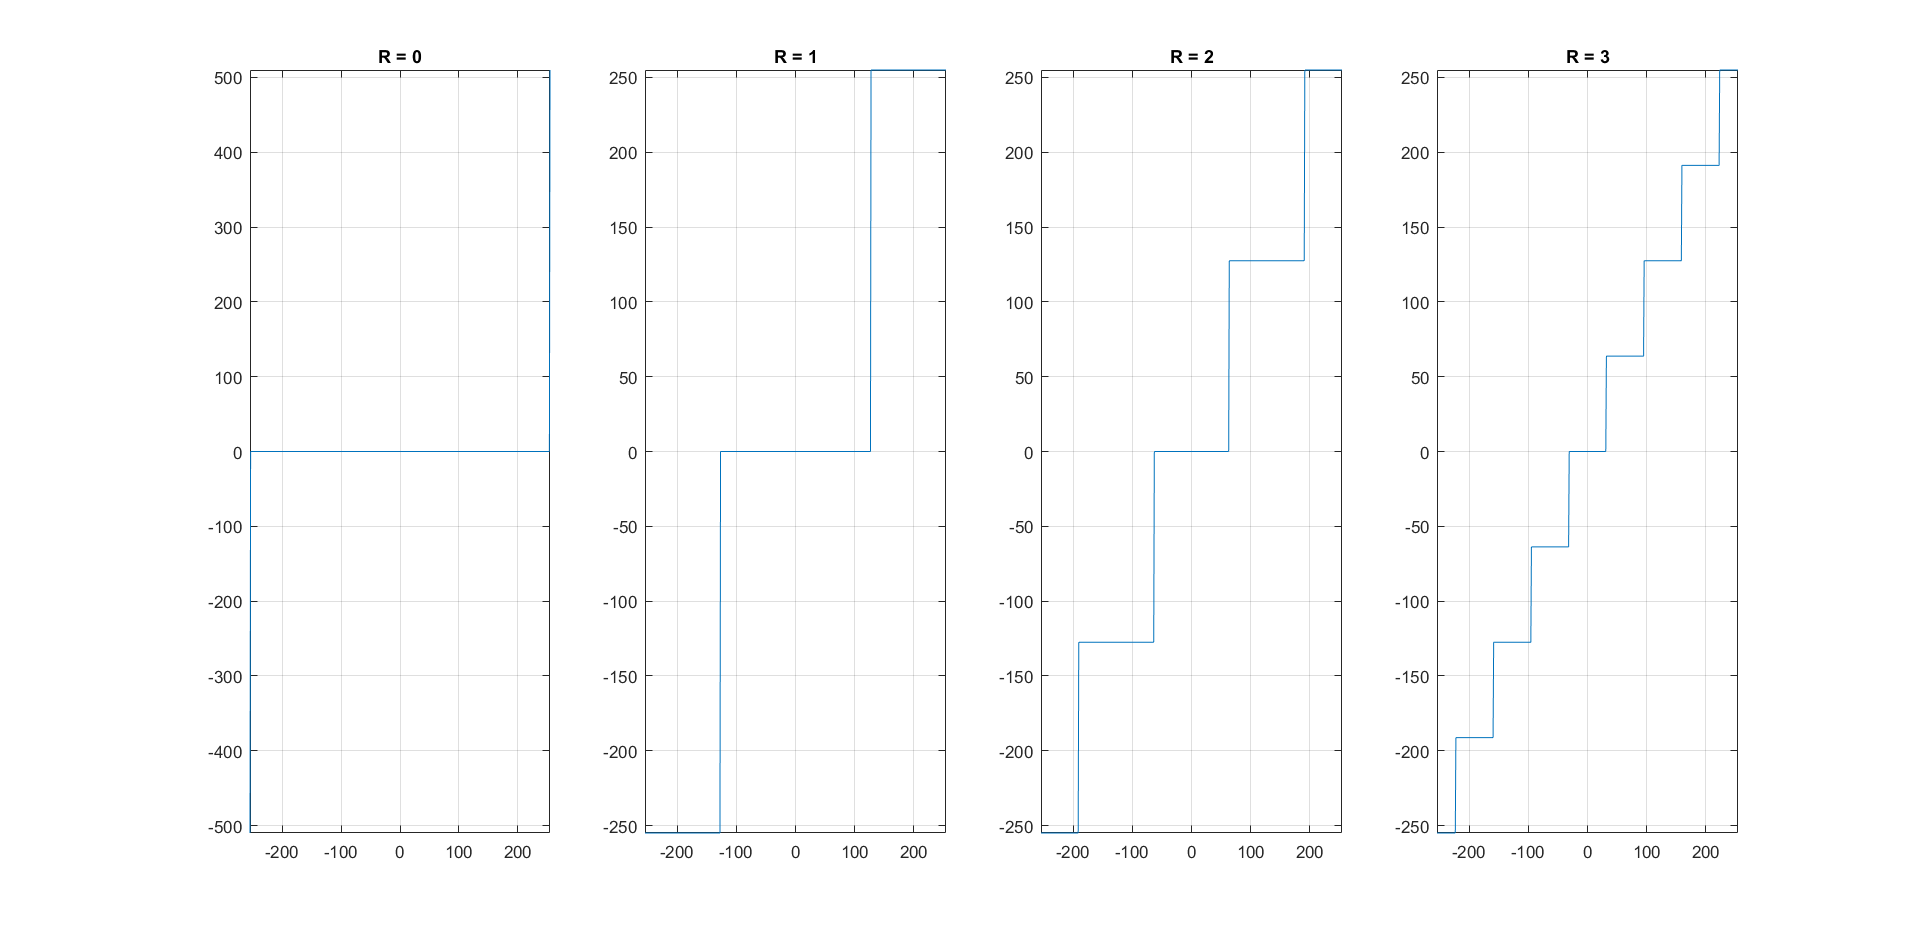
\includegraphics[height=4cm, width=\linewidth]{partA_quantizer_a.png}
		\end{subfigure}%
		~
		\begin{subfigure}[t]{0.5\textwidth}
			\centering
			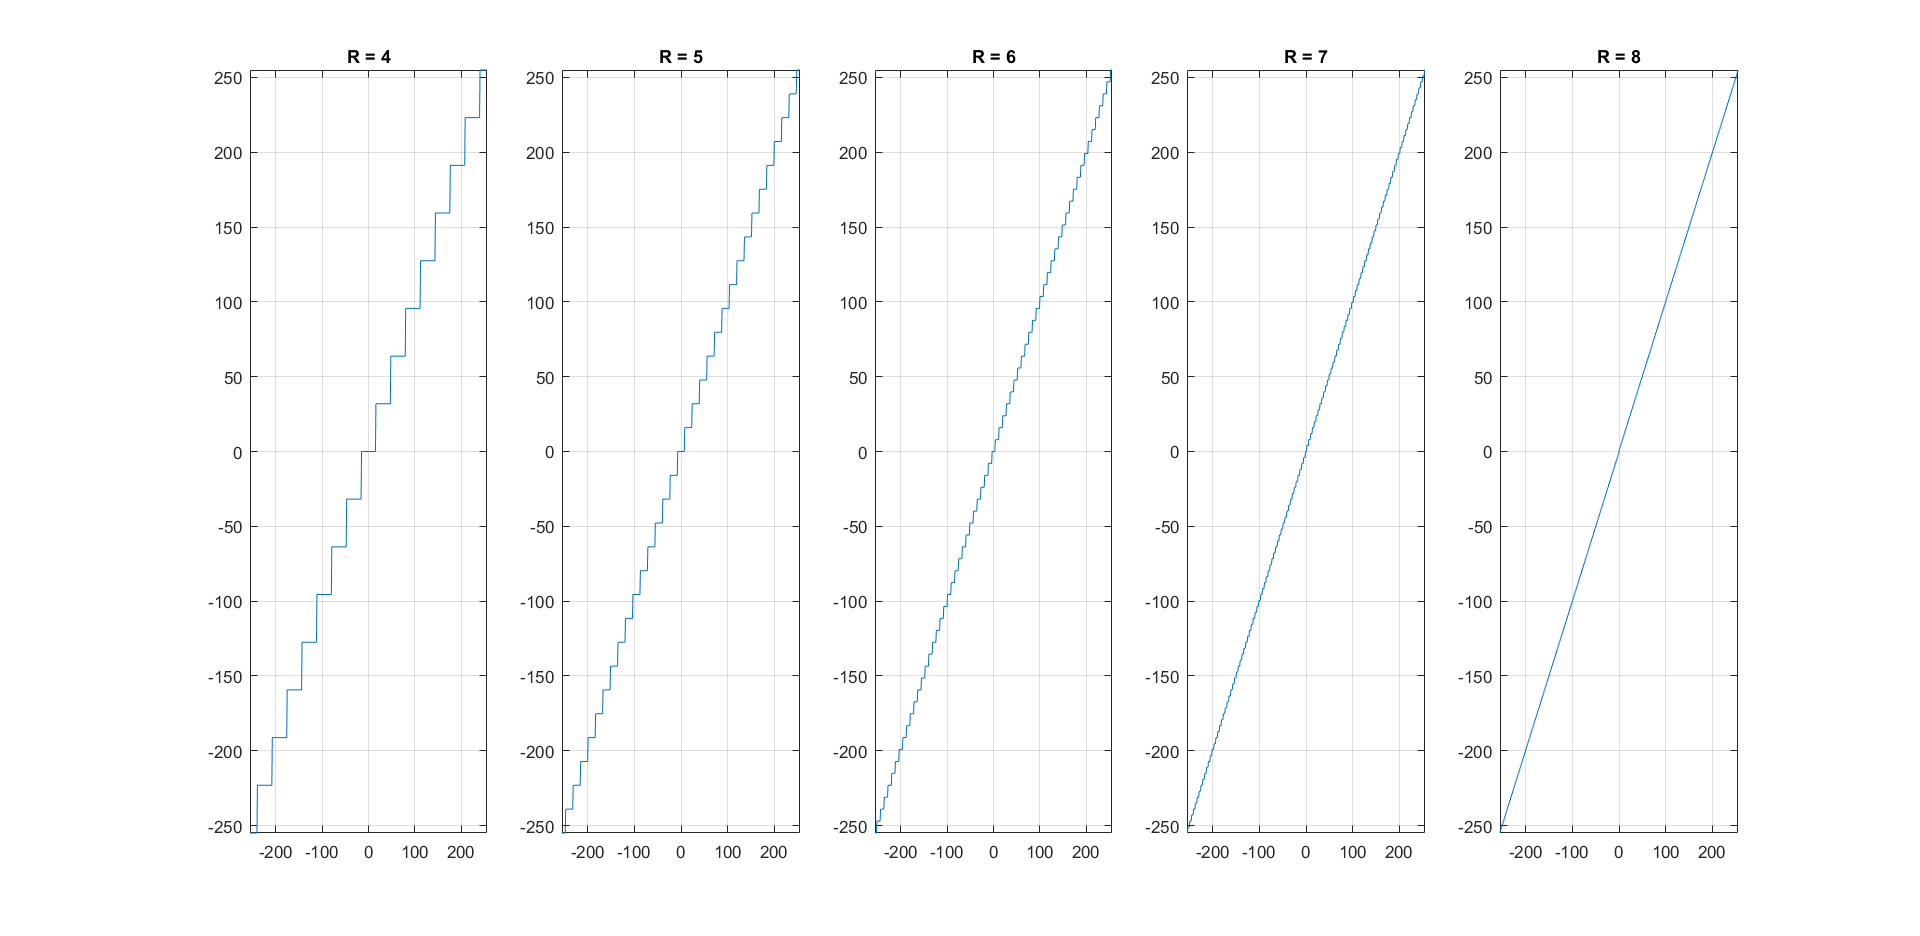
\includegraphics[height=4cm, width=\linewidth]{partA_quantizer_b.png}
		\end{subfigure}
	\end{figure}
	
	\noindent
	Όπως παρατηρούμε από τις παραπάνω εικόνες, καθώς αυξάνεται η τιμή της παραμέτρου R, αυξάνονται τα επίπεδα κβάντιστης, ενώ μειώνεται το μήκος του κάθε διαστήματος Δ. Αποτέλεσμα αυτού είναι ότι με την αύξηση του R έχουμε περισσότερες τιμές Q(x) που αντιστοιχούν στην είσοδο x και έτσι με την κβάντιση δεν έχουμε μεγάλες απώλειες-διαφορές από το σήμα εισόδου.\\
	
	\noindent
	Στη συνέχεια, χρησιμοποιώντας τη συνάρτηση "uni\_scalar", μας ζητήθηκε να κβαντίσουμε την εικόνα "lena\_gray\_512.tif". Για να γίνει σωστά η κβάντιση, μετατράπηκε η εικόνα σε ένα vector και έπειτα για το ίδιο έυρος τιμών της παραμέτρου R έγινε η κβάντιση. Επιπλέον, μετρήθηκε και το MSE, για να υπολογίσουμε αν υπάρχουν μεγάλες απώλειες κατά την διαδικασία της κβάντισης.
	
	\begin{figure}[h!]
	 	\centering
	 	\begin{subfigure}[t]{0.5\textwidth}
	 		\centering
	 		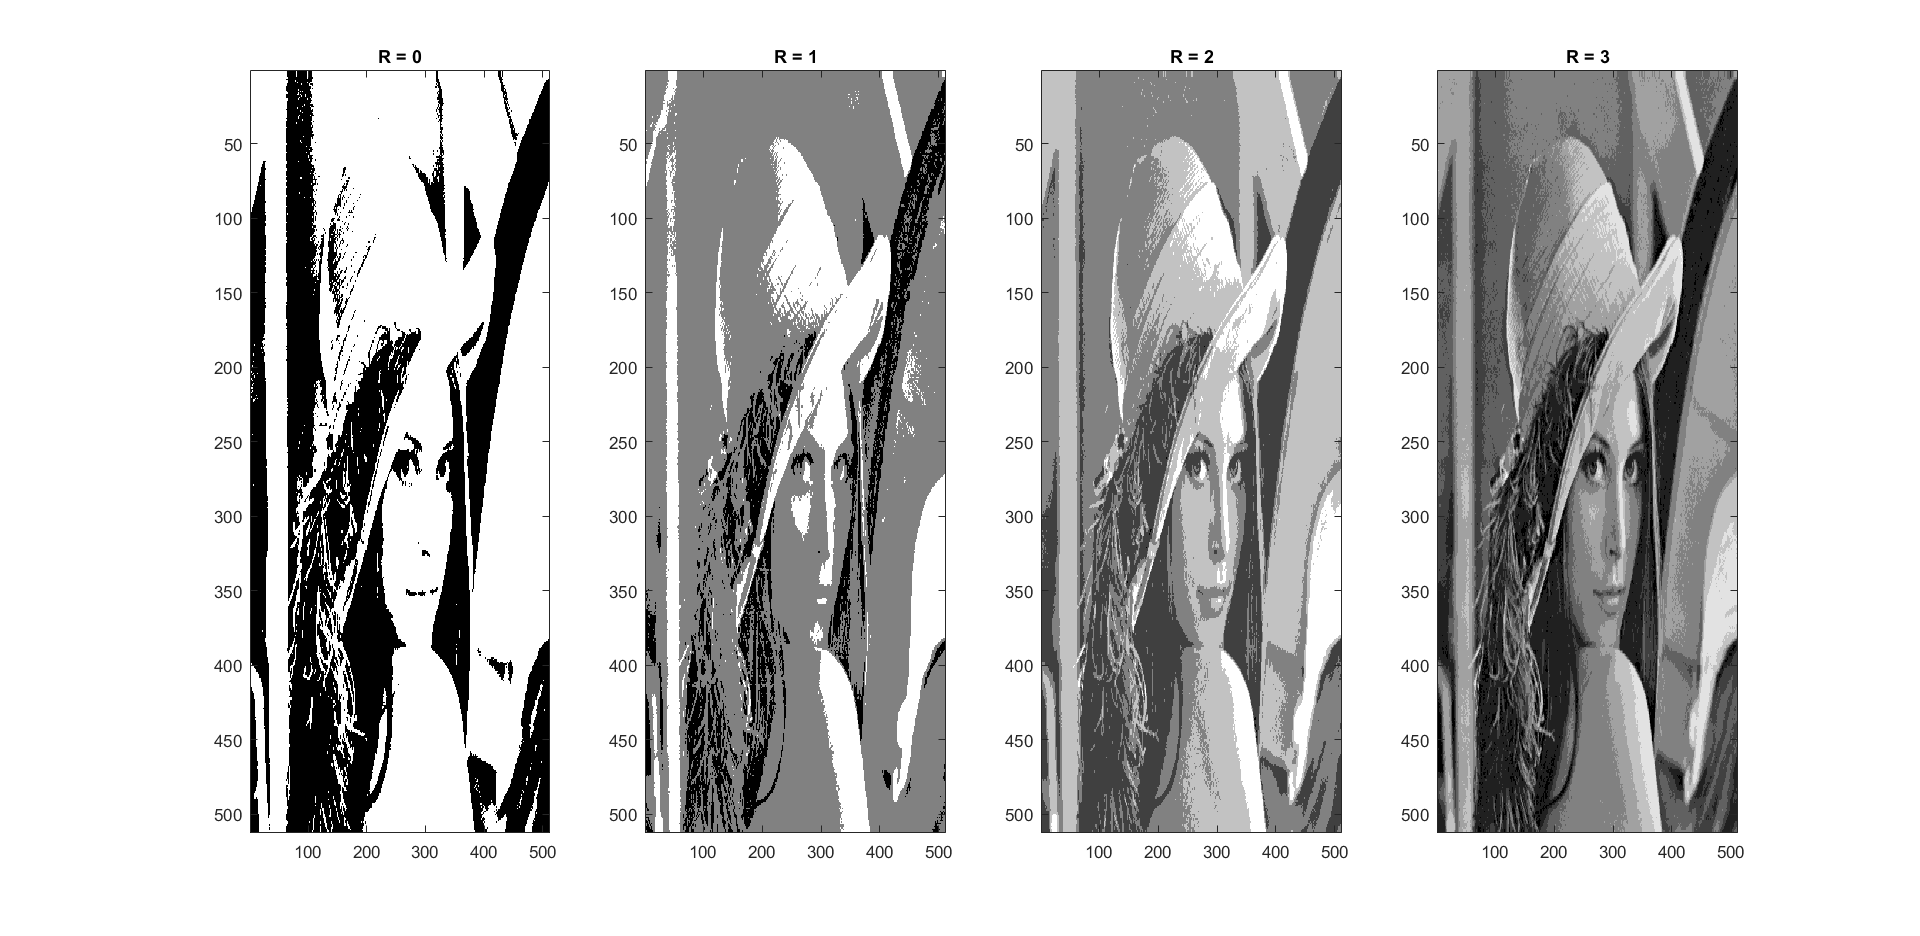
\includegraphics[height=5cm, width=\linewidth]{partA_lena_a.png}
	 	\end{subfigure}%
	 	~
	 	\begin{subfigure}[t]{0.5\textwidth}
	 		\centering
	 		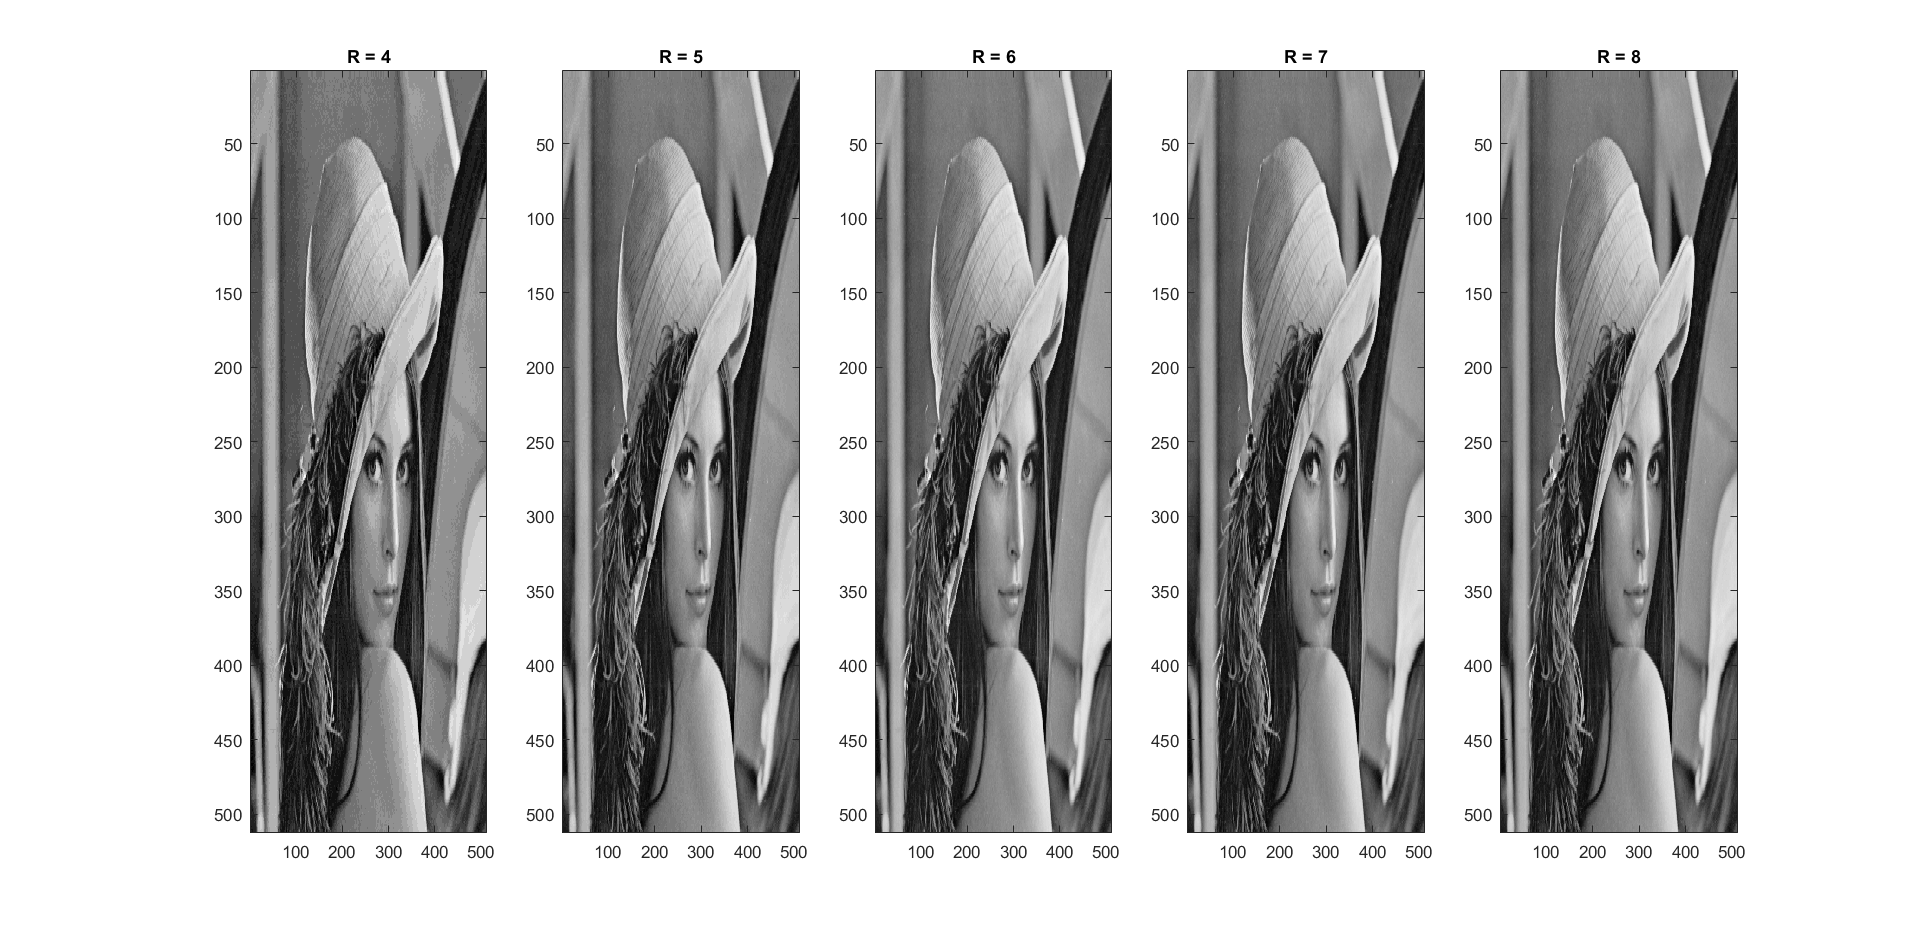
\includegraphics[height=5cm, width=\linewidth]{partA_lena_b.png}
	 	\end{subfigure}
	\end{figure}

	\noindent
	Για κάθε τιμή της παραμέτρου R έχουμε τα παρακάτω MSE για την εικόνα.\\
	\begin{table}[h!]
		\centering
		\begin{tabular}{|c|c|c|c|c|c|c|c|c|}
			\hline
			R=0 & R=1 & R=2 & R=3 & R=4 & R=5 & R=6 & R=7 & R=8 \\
			\hline
			5325,7372 & 1170,6221 & 228,5398 & 66,3848 & 15,9621 & 3,9335 & 0,9874 & 0,2459 & 0,0617 \\
			\hline
		\end{tabular}
	\end{table}

	\pagebreak
	\noindent
	Από τις παραπάνω εικόνες παρατηρούμε ότι για R = 0 η εικόνα είναι binary και καθώς αυξάνεται έχουμε ακόμα περισσότερους τόνους του γκρι και περισσότερη λεπτομέρεια στην εικόνα. Επιπλέον, από τον πίνακα με τα MSE, βλέπουμε ότι με την αύξηση του R μειώνεται το error, επειδή έχουμε περισσοτερα επίπεδα κβάντισης με αποτέλεσμα να έχουμε περισσότερους τόνους του γκρι στην εικόνα και να μην υπάρχουν μεγάλες απώλειες-διαφορές εξαιτίας της κβάντισης. \\
	
	\noindent
	Παρακάτω παρουσιάζεται το διάγραμμα Rate-Distortion. \\
	\begin{figure}[h!]
		\centering
		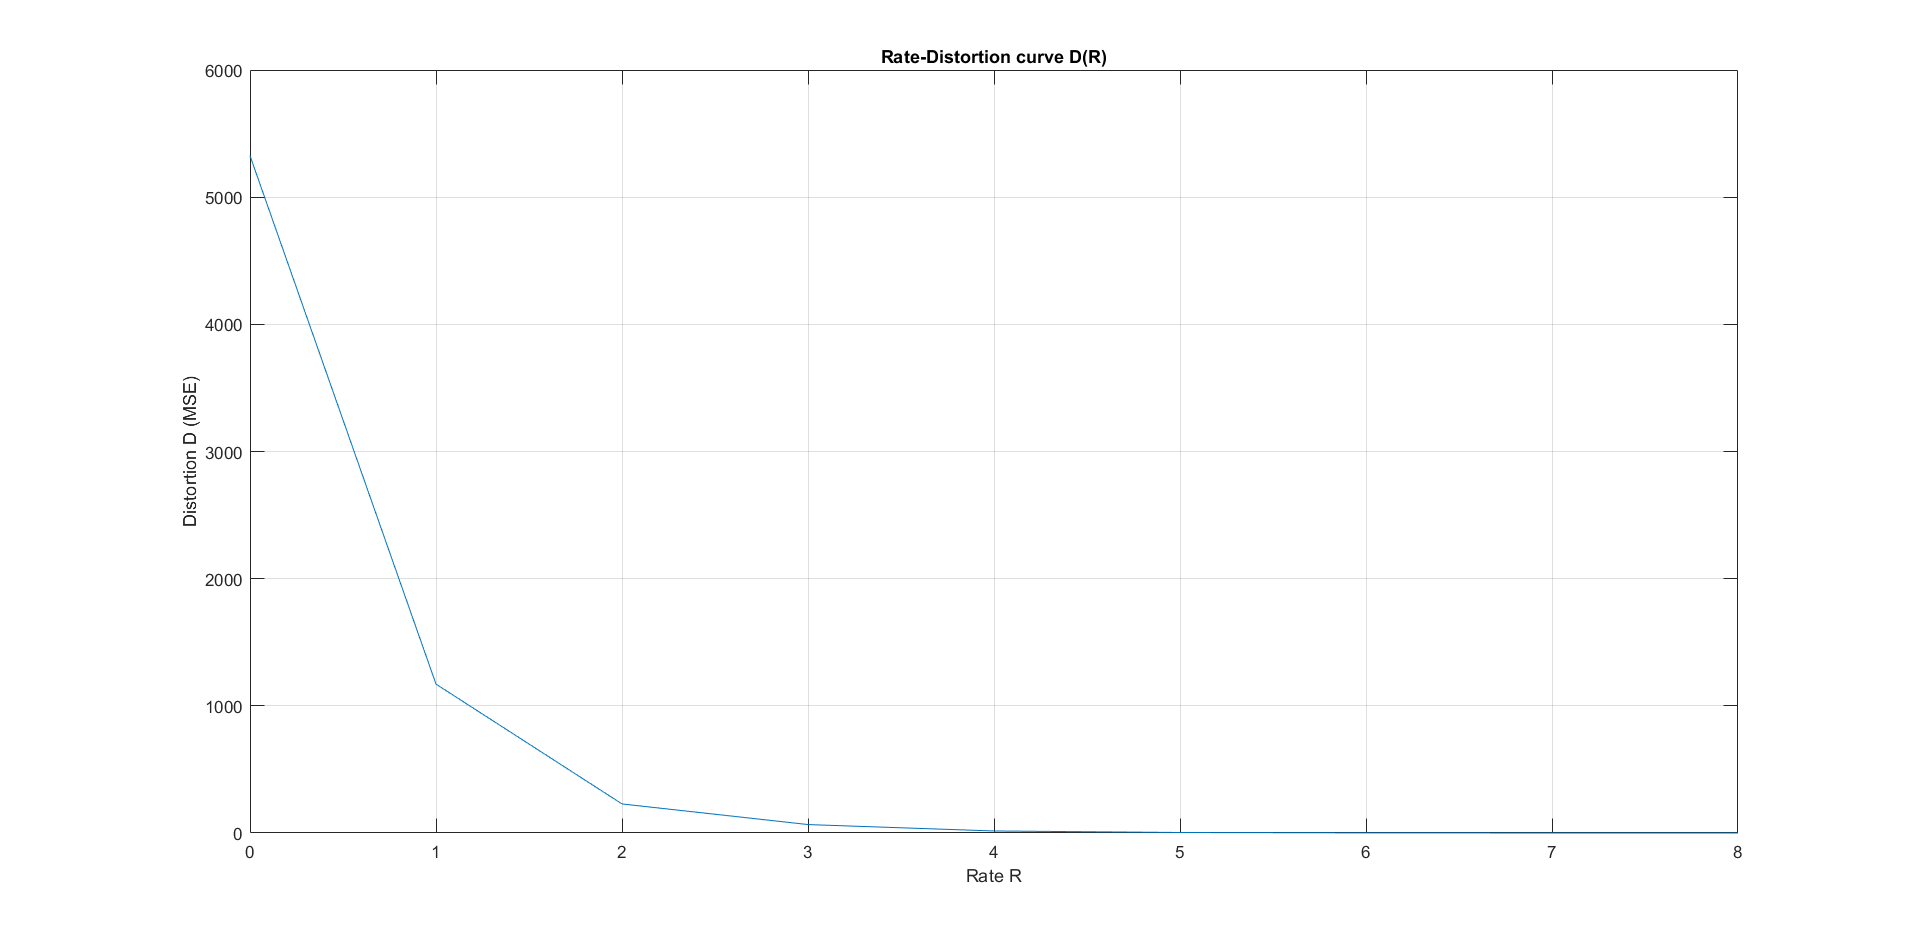
\includegraphics[height=5cm,width=10cm]{partA_rate_distortion.png}
	\end{figure}

	\noindent
	Όπως φαίνεται βλέπουμε ότι το distortion μειώνεται με την αύξηση του R, δηλαδή το MSE της εικόνας μειώνεται για τους λόγους που αναφέρθηκαν παραπάνω.
	
\section*{Part B}
	Σκοπός του δεύτερου μέρους της εργασίας είναι να επεξεργαστούμε ένα βίντεο. Το βίντεο που θέλουμε να επεξεργαστούμε είναι το "xylophone.mp4", από το οποίο θα πρέπει να εξάγουμε κάποιες πλήροφορίες που αφορούν το frame rate, τον αριθμό των frames, την ανάλυση του κάθε frame και τη συνολική διάρκεια του βίντεο. Γι' αυτό το λόγο χρησιμοποιήθηκαν οι συναρτήσεις hasFrame(), readFrame() και pause().  
	
	\noindent
	Παρακάτω παρουσιάζονται τα δεδομένα που μας ζητήθηκαν να βρούμε.
	
	\begin{table}[h!]
		\centering
		\begin{tabular}{|c|c|c|c|}
			\hline
		Total Duration (sec) & Frame Rate (frames/sec) & Total Frames & Resolution \\
			\hline
			4.7 & 30 & 141 & 140x320 \\
			\hline
		\end{tabular}
	\end{table}

	\noindent
	Όσον αφορά την εξαγωγή του πεντηκοστού frame του βίντεο, χρησιμοποιήθηκε η συνάρτηση imwrite(), ενώ στη συνέχεια για να γίνει ασπρόμαυρη η εικόνα χρησιμοποιήθηκεη συνάρτηση rgb2gray(). Tα αποτελέσματα που προέκυψαν είναι τα εξής:
	
	\begin{figure}[h!]
		\centering
		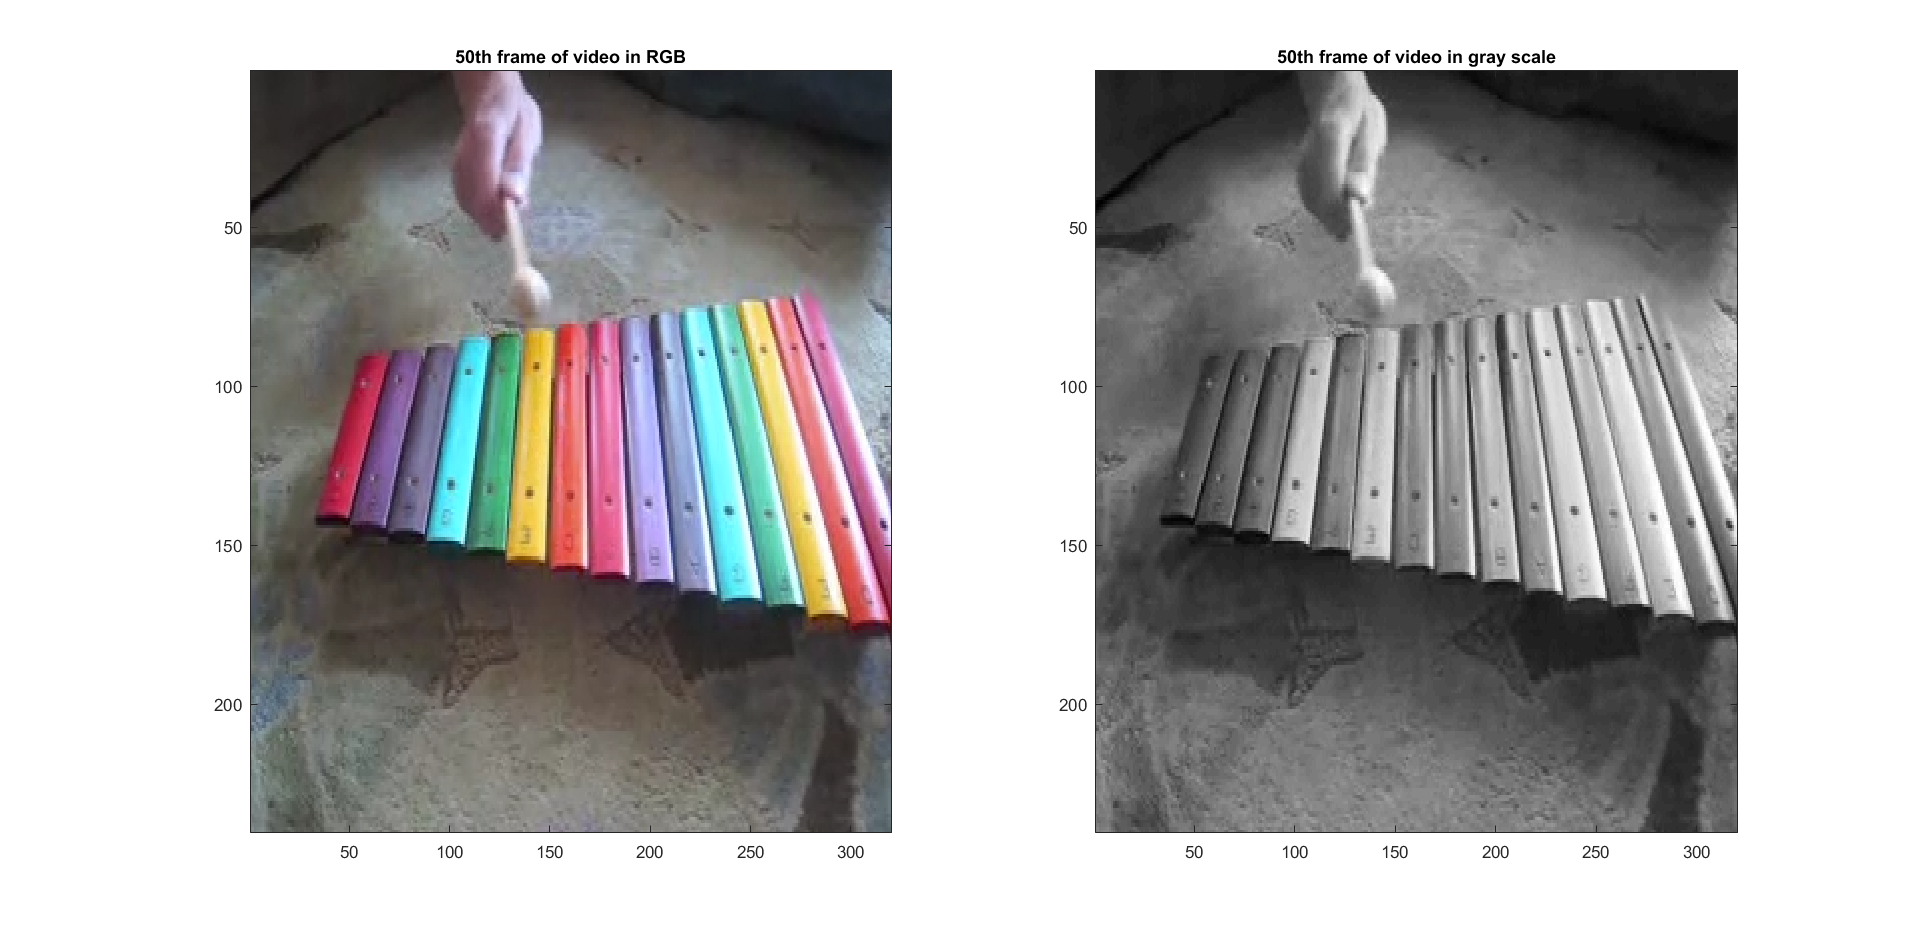
\includegraphics[height=6cm,width=12cm]{partB_xylophone.png}
	\end{figure}
\pagebreak
\section*{Part C}
	Σκοπός του τρίτου και τελευταίου μέρους της εργασίας είναι να κατασκευάσουμε ένα σύστημα συμπίεσης μιας εικόνας χρησιμοποιώντας το μετασχηματισμό Haar και τον κβαντιστή που υλοποιή- \\θηκε στο πρώτο μέρος της εργασίας. Για το λόγο αυτό υλοποιήθηκε μια συνάρτηση που υπολογίζει τον μετασχηματισμό Haar ενός 1D σήματος και τον αντίστροφο μετασχηματισμό. Kατόπιν, έγινε ένα resize στην εικόνα σε διαστάσεις 256x256. Επιπλέον, για την εφαρμογή του Haar στην εικόνα, εφαρμόζουμε πρώτα το μετασχηματισμό τις γραμμες και στο αποτέλεσμα που προκύπτει εφαρμόζουμε πάλι τον Haar στις στήλες. Tην ίδια διαδικασία εφαρμόζουμε στις χαμηλές συχνότητες (HH) για δεύτερη φορά για την κατασκευή δύο επιπέδων Haar. Στη συνέχεια, κβαντίζουμε για R=4 όλα τα subbands εκτός από τις χαμηλές συχνότητες και προκύπτουν τα παρακάτω αποτελέσματα.
	
	\begin{figure}[h!]
		\centering
		\begin{subfigure}[t]{0.5\textwidth}
			\centering
			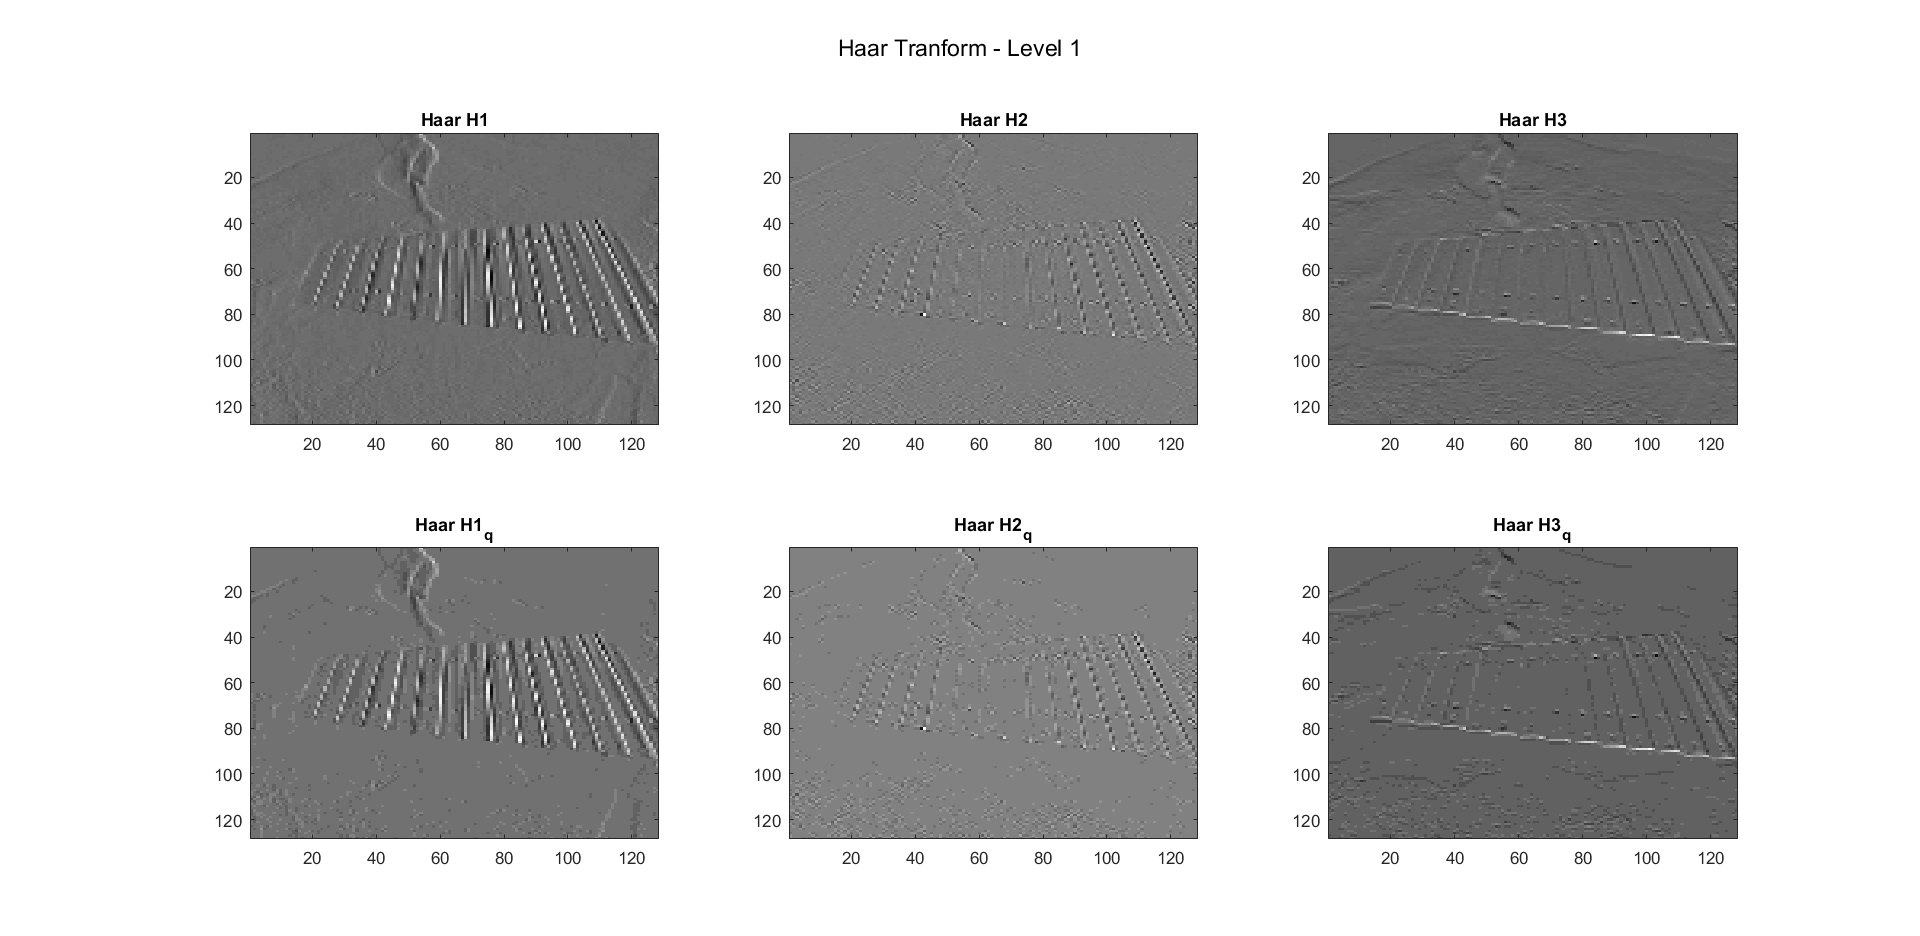
\includegraphics[height=5cm, width=\linewidth]{partC_lvl1_haartq1.png}
		\end{subfigure}%
		~
		\begin{subfigure}[t]{0.5\textwidth}
			\centering
			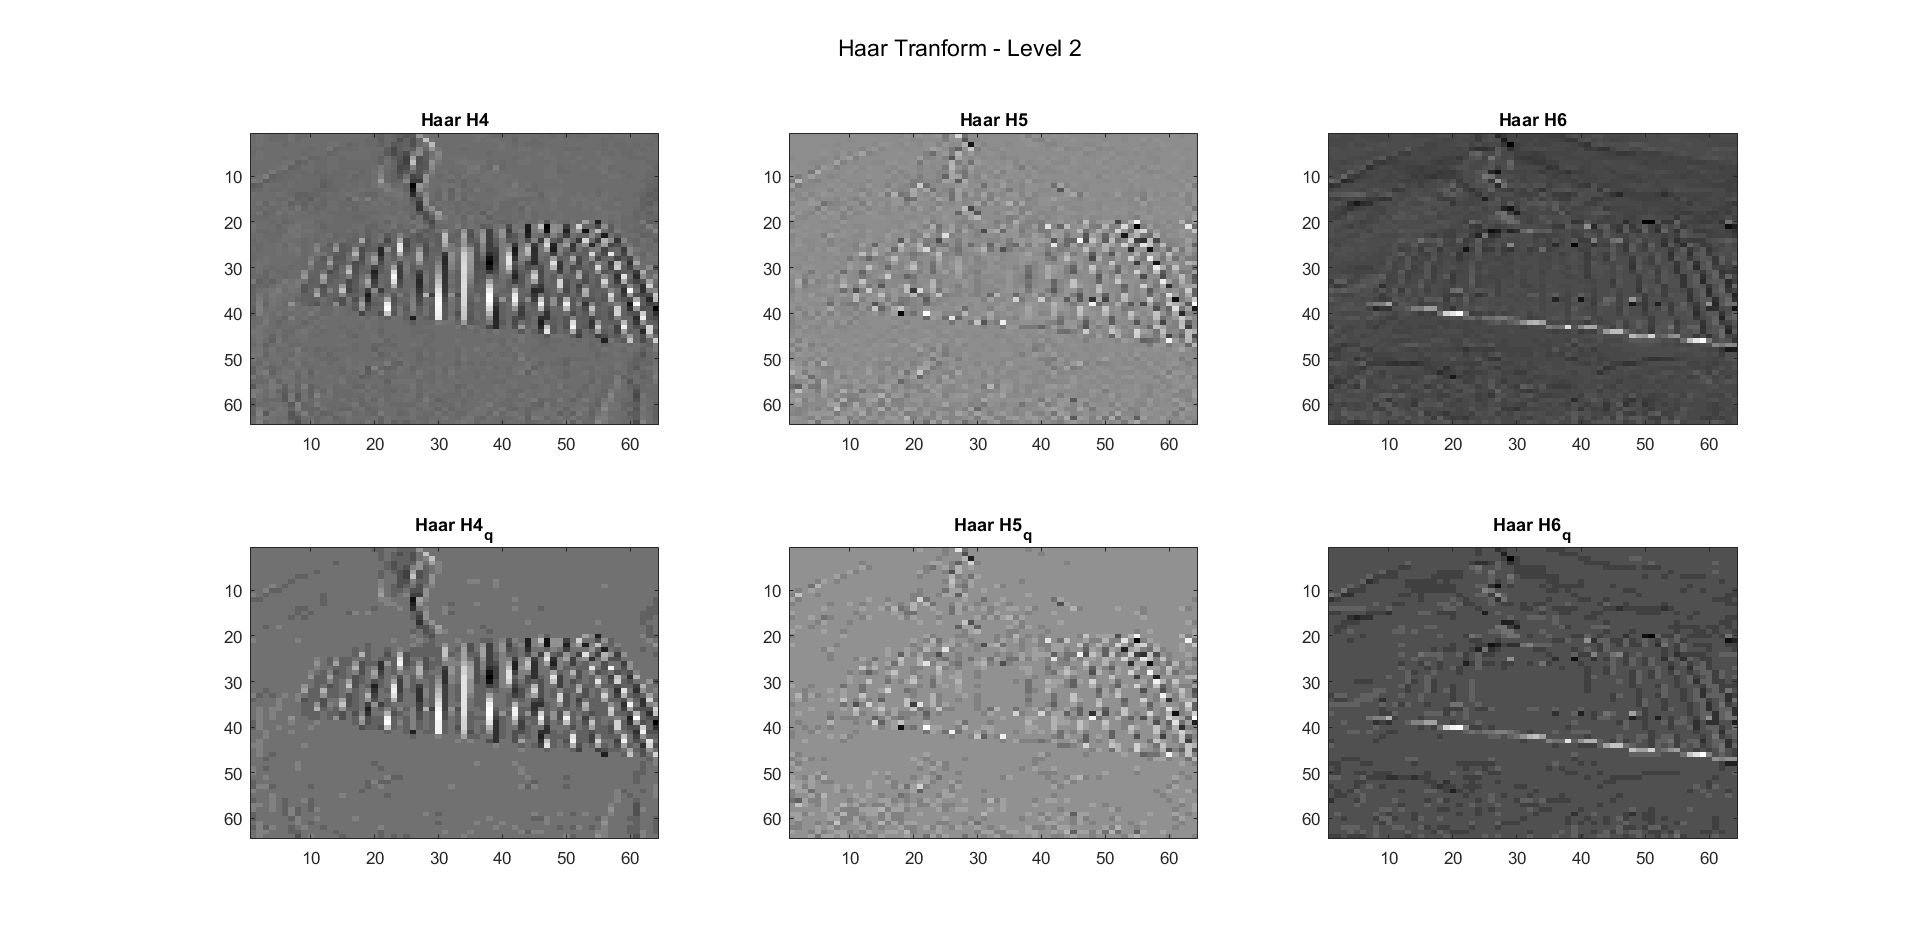
\includegraphics[height=5cm, width=\linewidth]{partC_lvl2_haartq1.png}
		\end{subfigure}
		\caption{Haar Subbands and quantized Subbands}
	\end{figure}

	\noindent
	Παρακάτω παρουσιάζεται ο μετασχηματισμός Haar (αριστερά) και ο μετασχηματισμός Haar με την κβαντιση των subbands για R=4 και στα δύο επίπεδα (δεξιά).
	
	\begin{figure}[h!]
		\centering
		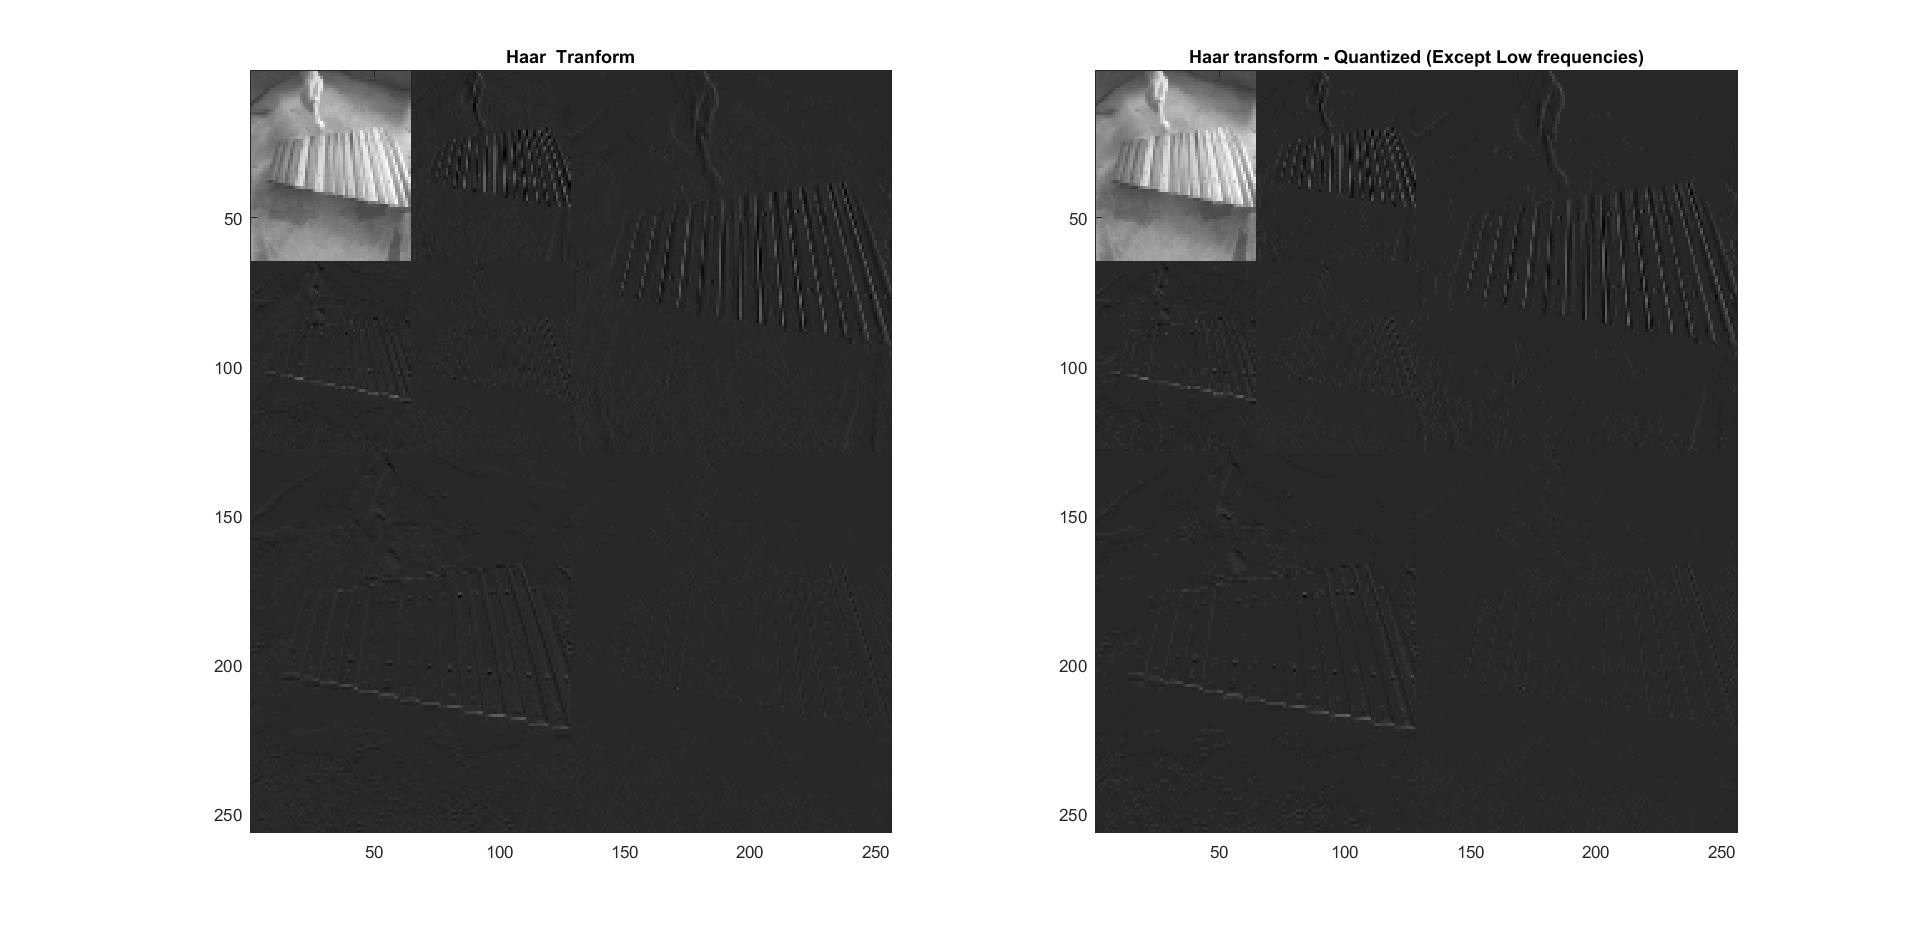
\includegraphics[height=5cm, width=\linewidth]{partC_haartq1.png}
	\end{figure}

	\pagebreak
	\noindent
	Στη συνέχεια, για τον υπολογισμό της εντροπίας, δημιουργήθηκαν τα παρακάτω ιστογράμματα του κάθε subband για τον υπολογισμό των πιθανοτήτων.
	
	\begin{figure}[h!]
		\centering
		\begin{subfigure}[t]{0.5\textwidth}
			\centering
			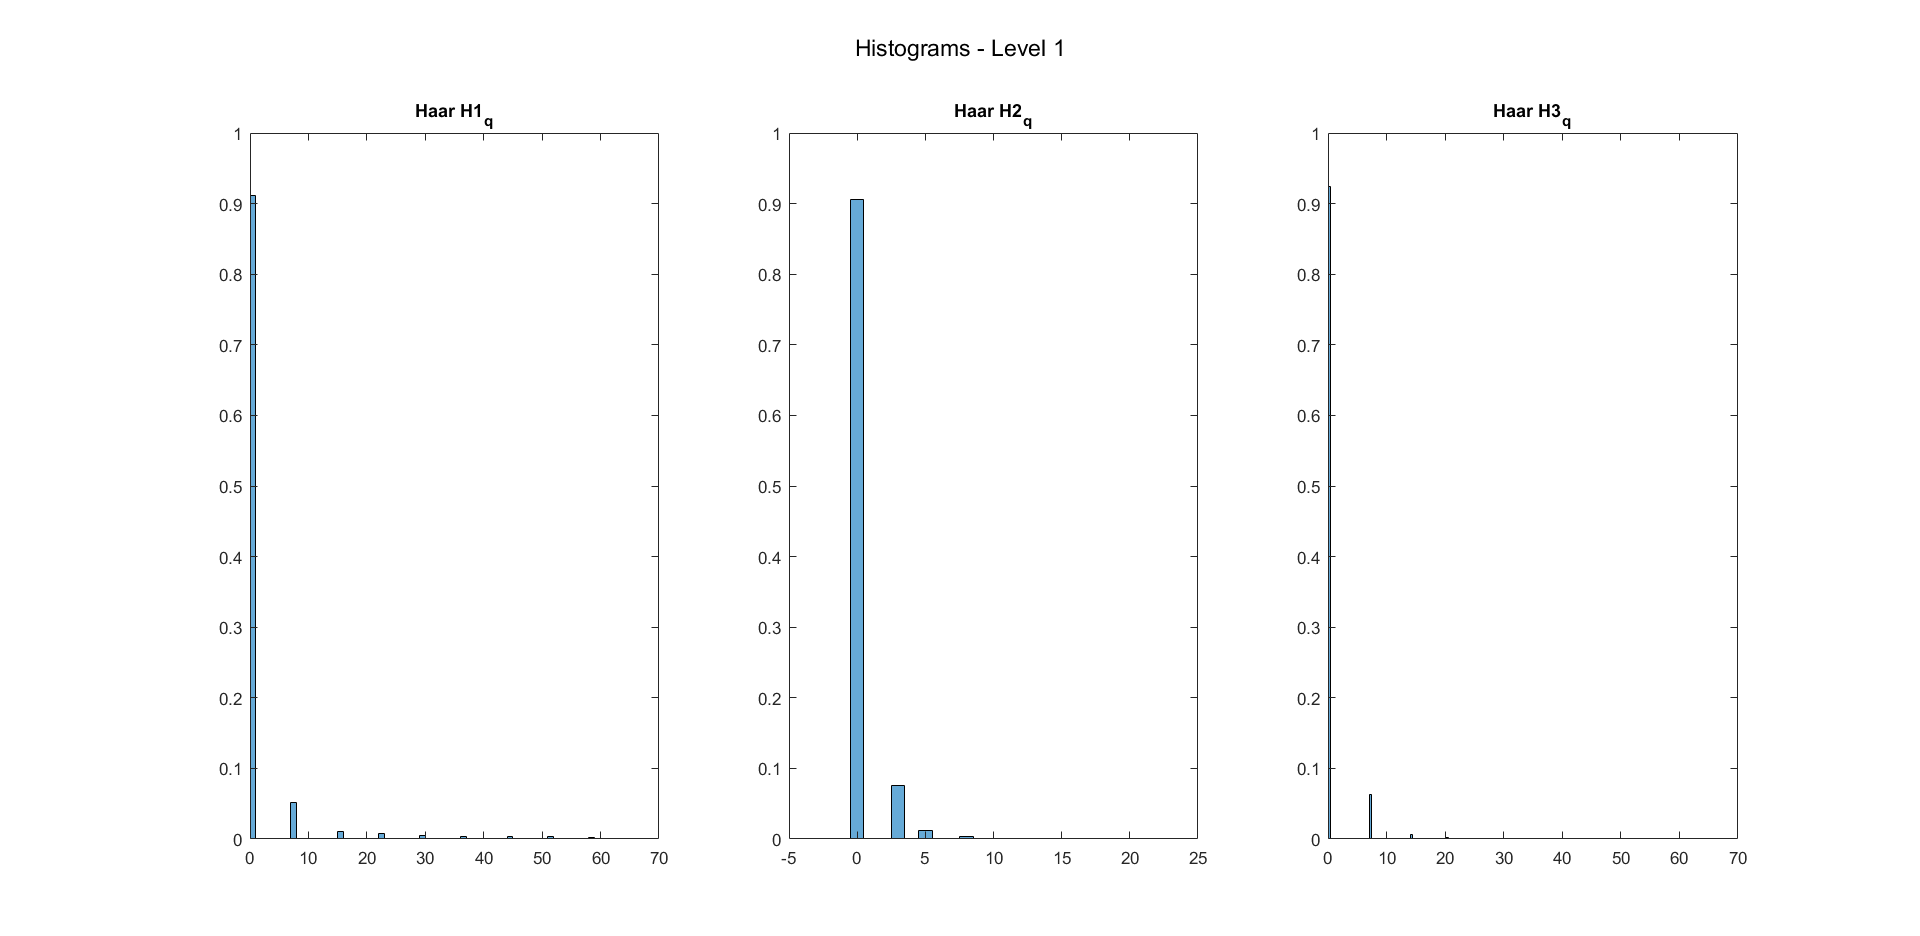
\includegraphics[height=4cm, width=\linewidth]{partC_lvl1_hists1.png}
		\end{subfigure}%
		~
		\begin{subfigure}[t]{0.5\textwidth}
			\centering
			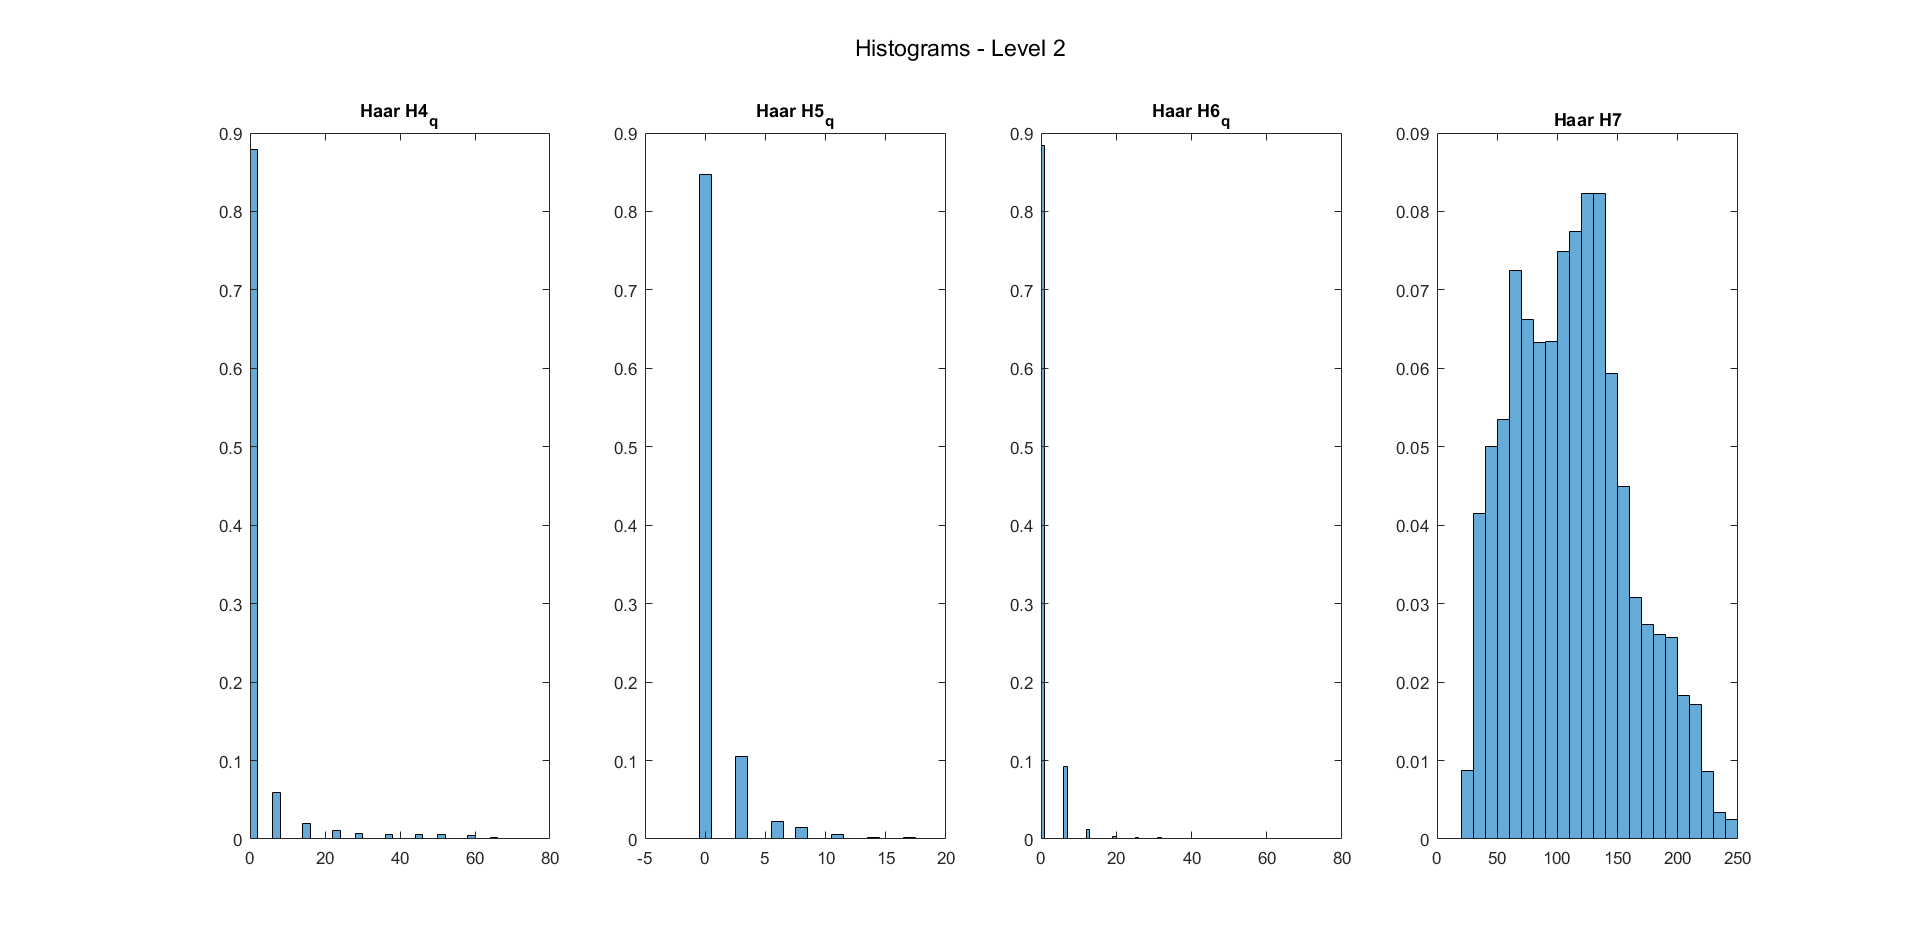
\includegraphics[height=4cm, width=\linewidth]{partC_lvl2_hists1.png}
		\end{subfigure}
	\end{figure}

	\noindent
	Αφού υπολογίστηκε η εντροπία κάθε κβαντισμένου subband, αθροίστηκαν ολες αυτές οι εντροπίες, για να προκύψει η συνολική της εικόνας μετά την εφαρμογή του μετασχηματισμού Haar και τη κβάντιση. Η συνολική τιμή της εντροπίας που προέκυψε για R=4 είναι 3.9434 bits/pixel.\\
	
	\noindent
	Στη συνέχεια, με τη συνάρτηση που κατασκευάστηκε για τον υπολογισμό του αντίστροφου μετασχηματισμού Haar, έγινε η ανακατασκευή της εικόνας. Επίσης, μετά την ανακατασκευή, μας ζητήθηκε να υπολογίσουμε το Peak SNR μέσω της συνάρηση psnr() της matlab. H τιμή του peak SNR είναι -10.774 ενώ το SNR είναι 31.0112 dB.\\
	
	\noindent
	Τέλος, μας ζητήθηκε να επαναλάβουμε την ίδια διαδικασία με τη διαφορά ότι αυτή τη φορά κβαντίζουμε το πρώτο επίπεδο Haar με R=3 και το δεύτερο επίπεδο με R=5.
	
	\begin{figure}[h!]
		\centering
		\begin{subfigure}[t]{0.5\textwidth}
			\centering
			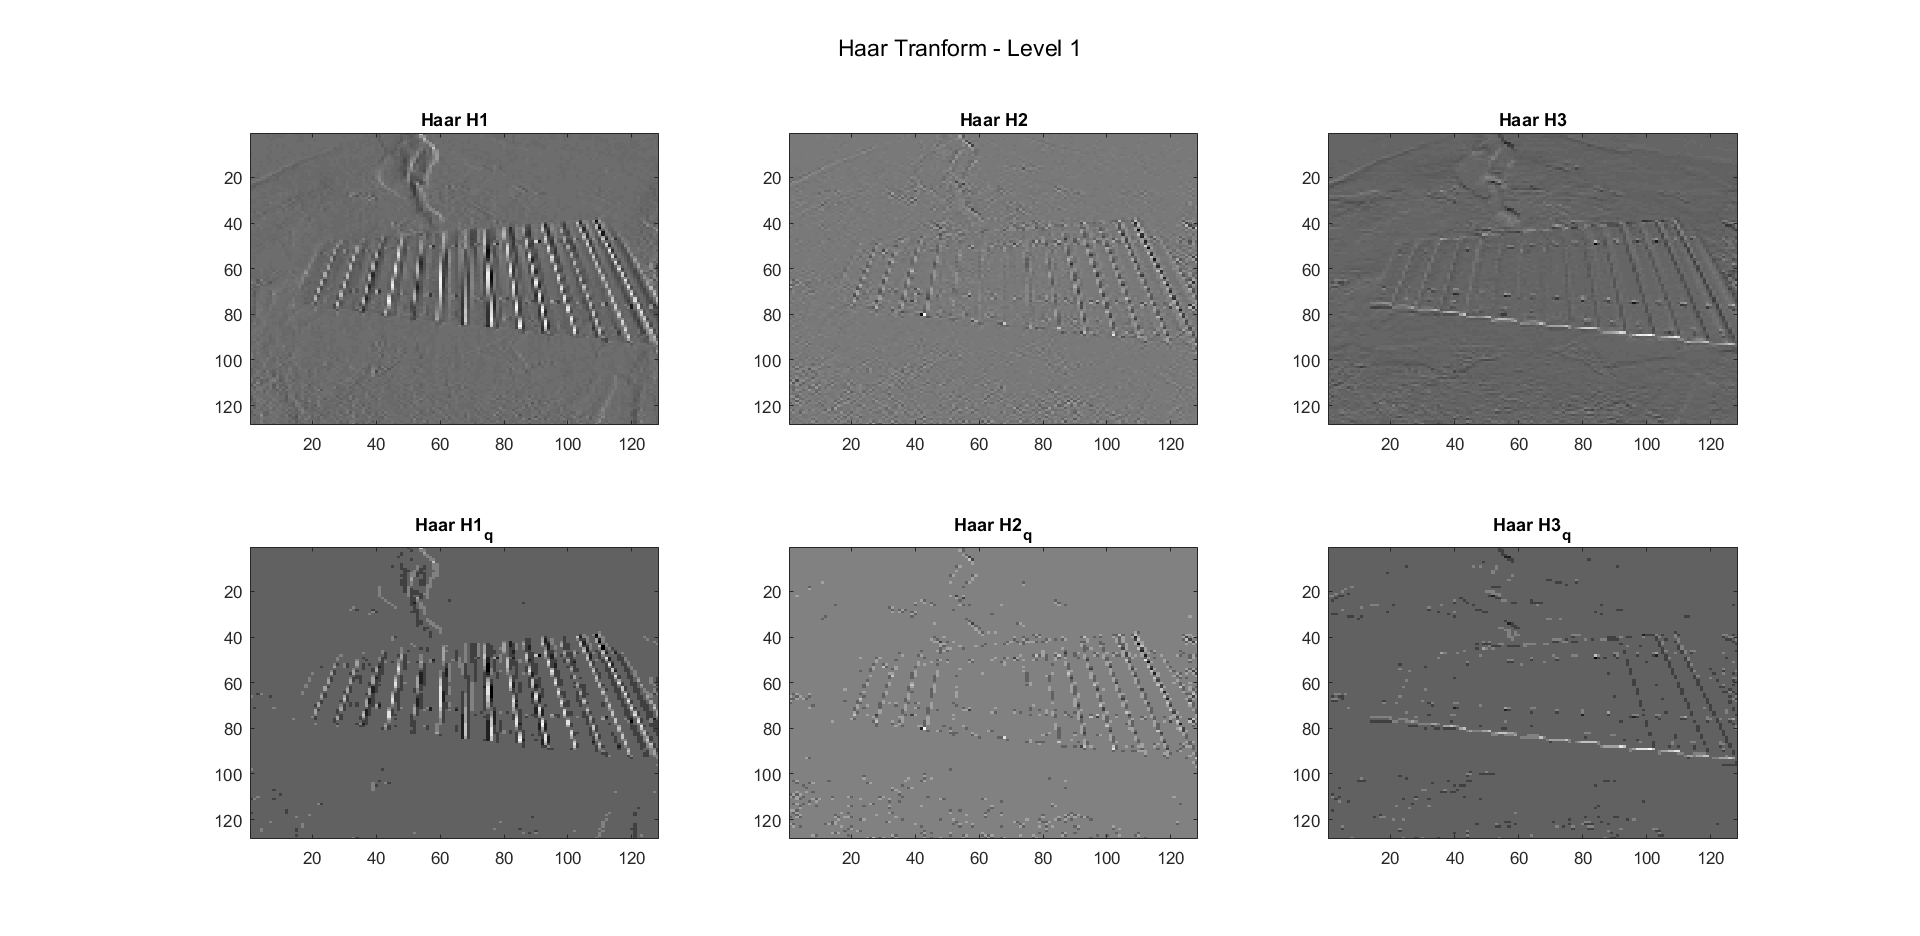
\includegraphics[height=5cm, width=\linewidth]{partC_lvl1_haartq2.png}
		\end{subfigure}%
		~
		\begin{subfigure}[t]{0.5\textwidth}
			\centering
			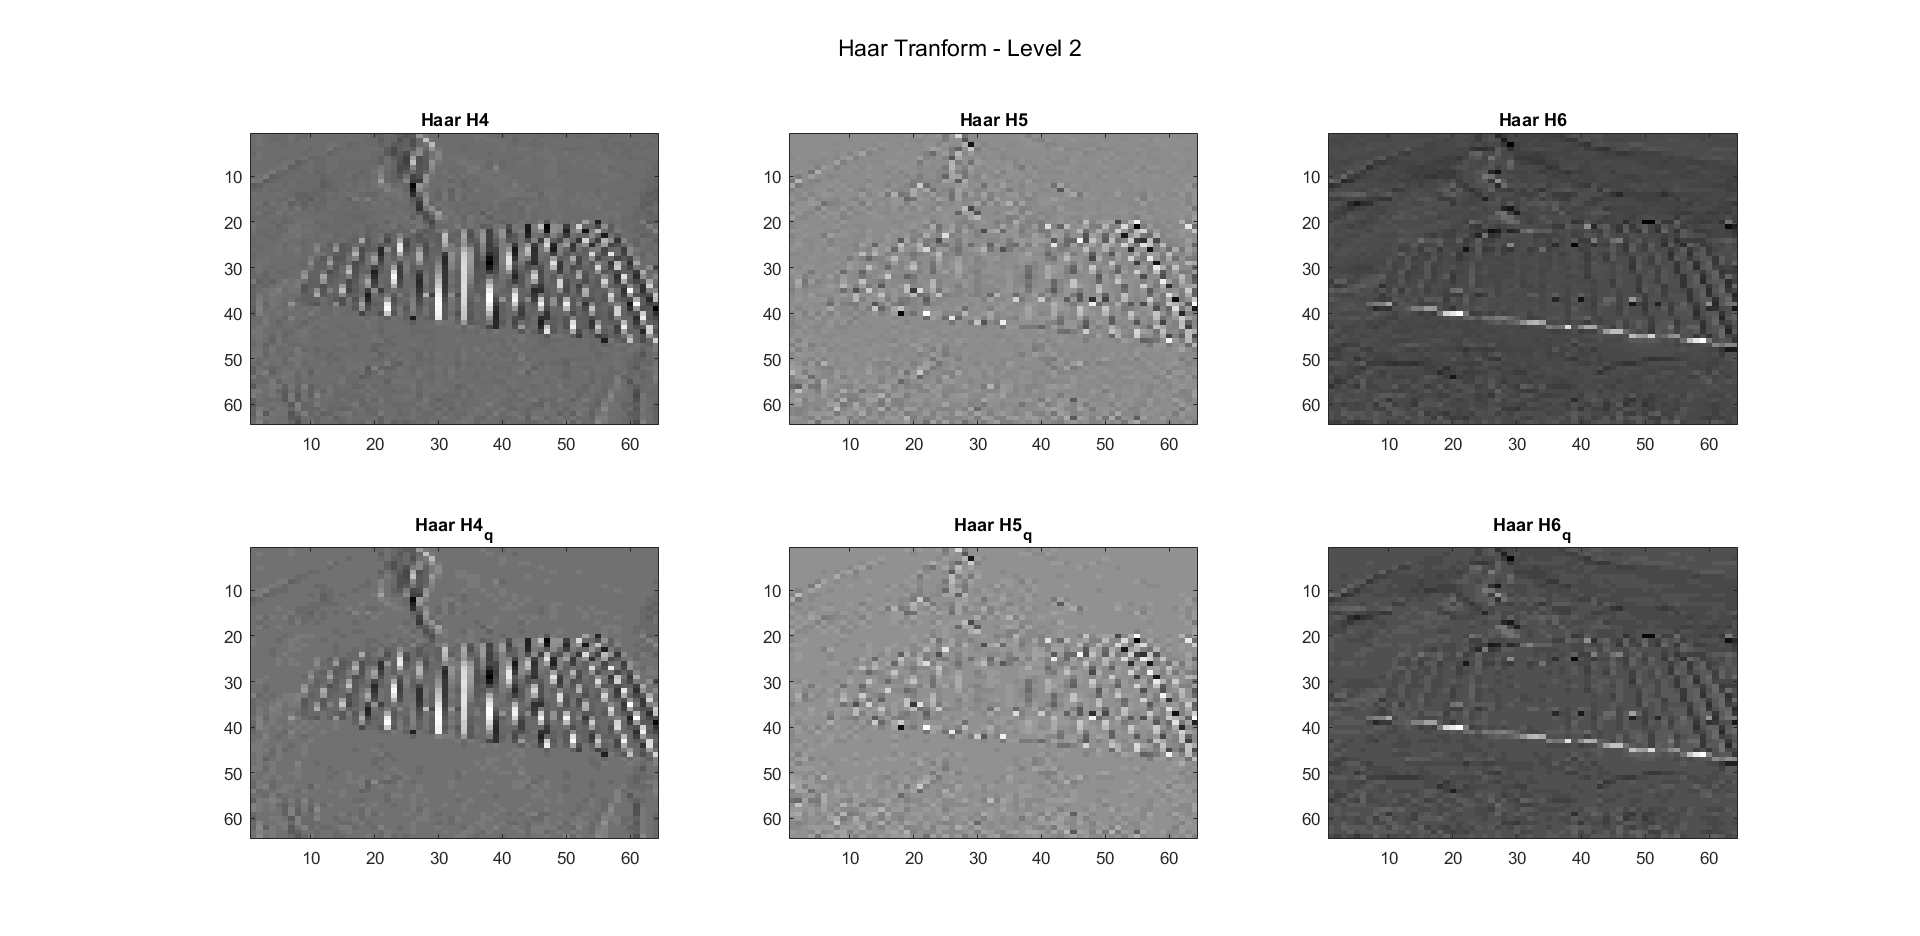
\includegraphics[height=5cm, width=\linewidth]{partC_lvl2_haartq2.png}
		\end{subfigure}
		\caption{Haar Subbands and quantized Subbands}
	\end{figure}	

	\noindent
	Από την παραπάνω εικόνα βλέπουμε ότι στο επίπεδο 1 λόγω του R=3 έχουμε λιγότερα επίπεδα κβάντισης με αποτέλεσμα να μειώνεται ακόμα περισσότερο η πληροφρία των subbands. Aντίθετα, στο επίπεδο 2 επειδή χρησιοποιούμε μεγαλύτερο R=5, έχουμε περισσότερη λεπτομέρεια σε αυτά τα subbands.\\
	
	\noindent
	Παρακάτω παρουσιάζεται ο μετασχηματισμός Haar (αριστερά) και ο μετασχηματισμός Haar με την κβαντιση των subbands για R=3 στο επίπεδο 1 και R=5 στο επίπεδο 2 (δεξιά).
		
	\begin{figure}[h!]
		\centering
		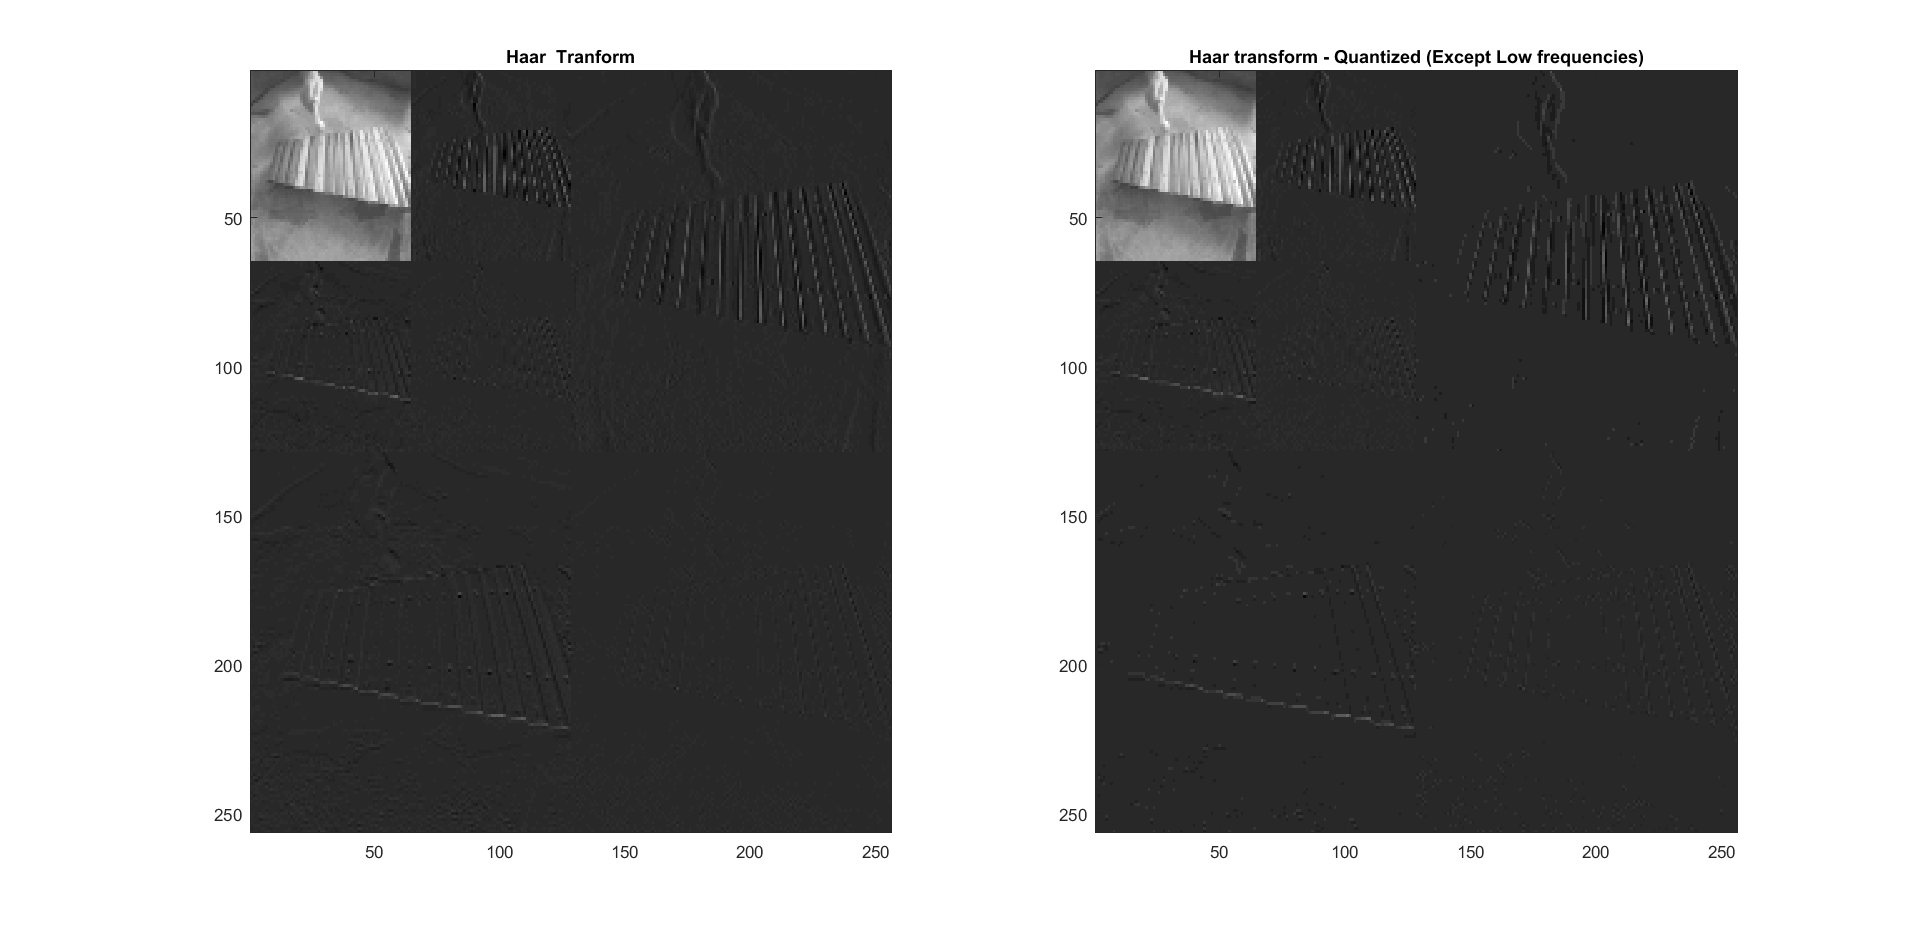
\includegraphics[height=4.5cm, width=\linewidth]{partC_haartq2.png}
	\end{figure}

	\pagebreak
	\noindent
	Όσον αφορά τα ιστογράμματα βλέπουμε ότι στο πρώτο επίπεδο εχουν μειωθεί οι τιμές που αντιστοιχούν σε κάθε επίπεδο κβάντισης, ενώ στο δεύτερο έχουν αυξηθεί, γεγονός που επαληθεύει και την ανάλυση κάθε εικόνας subband.
	
	\begin{figure}[h!]
		\centering
		\begin{subfigure}[t]{0.5\textwidth}
			\centering
			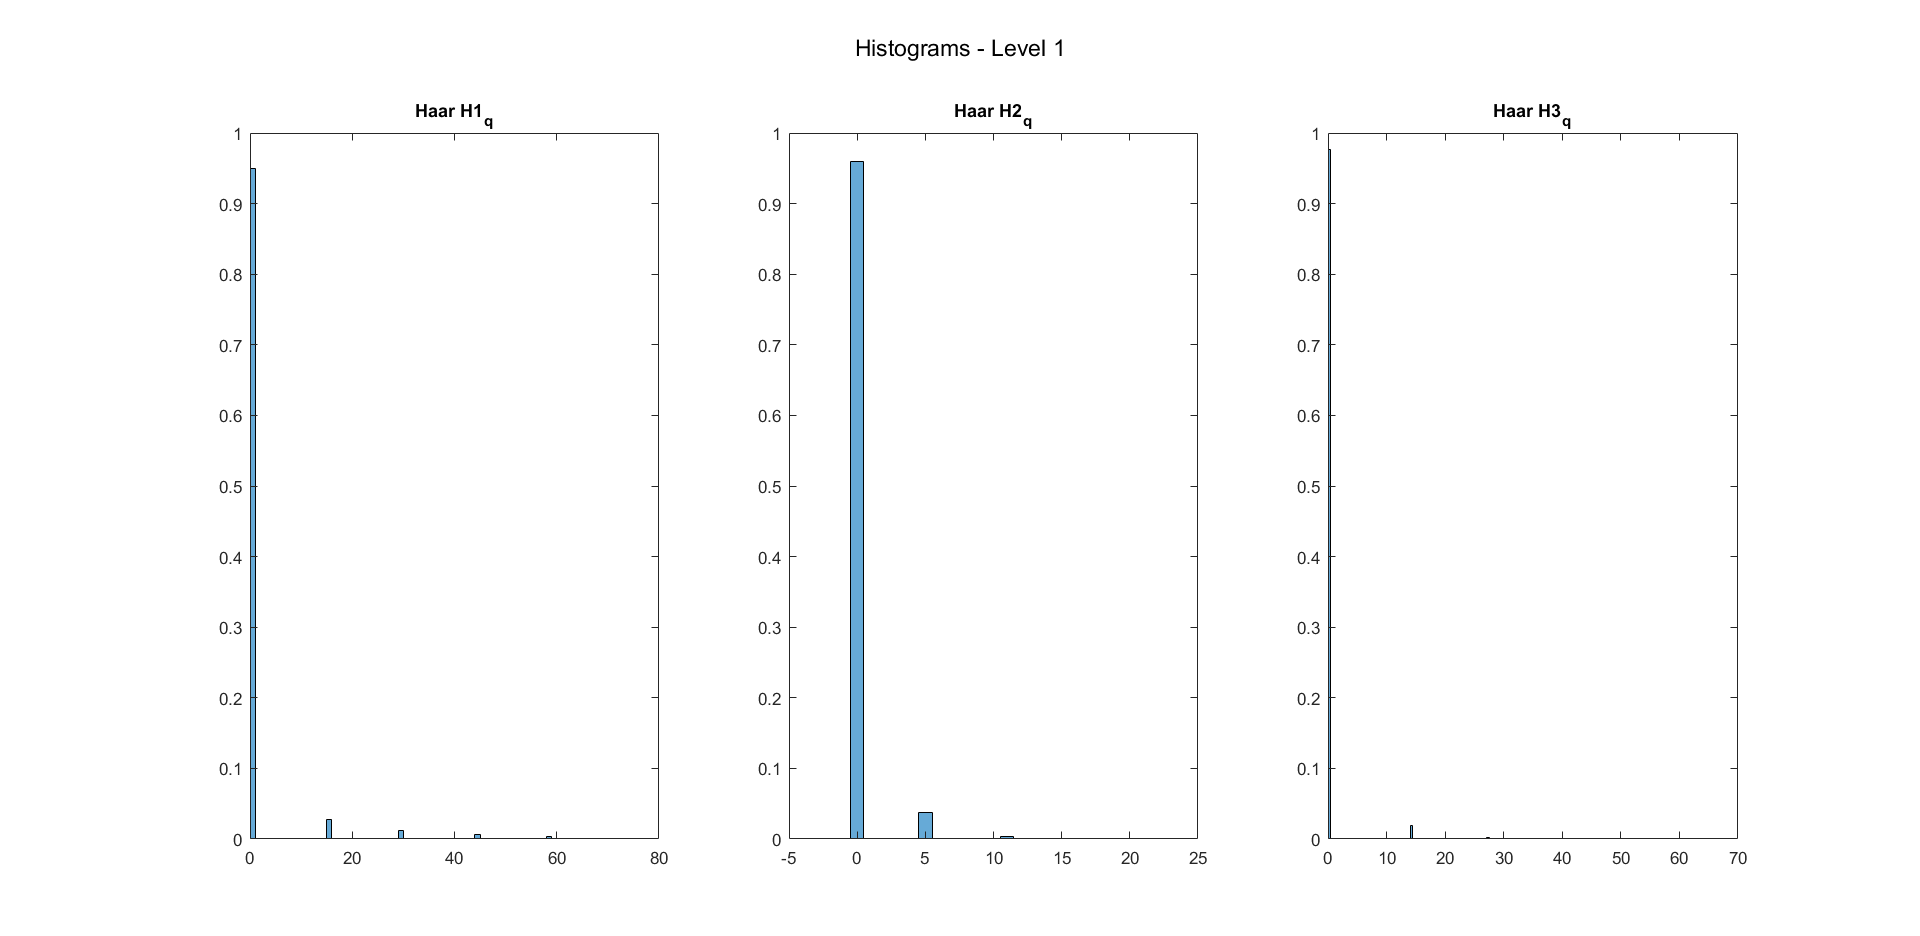
\includegraphics[height=5cm, width=\linewidth]{partC_lvl1_hists2.png}
		\end{subfigure}%
		~
		\begin{subfigure}[t]{0.5\textwidth}
			\centering
			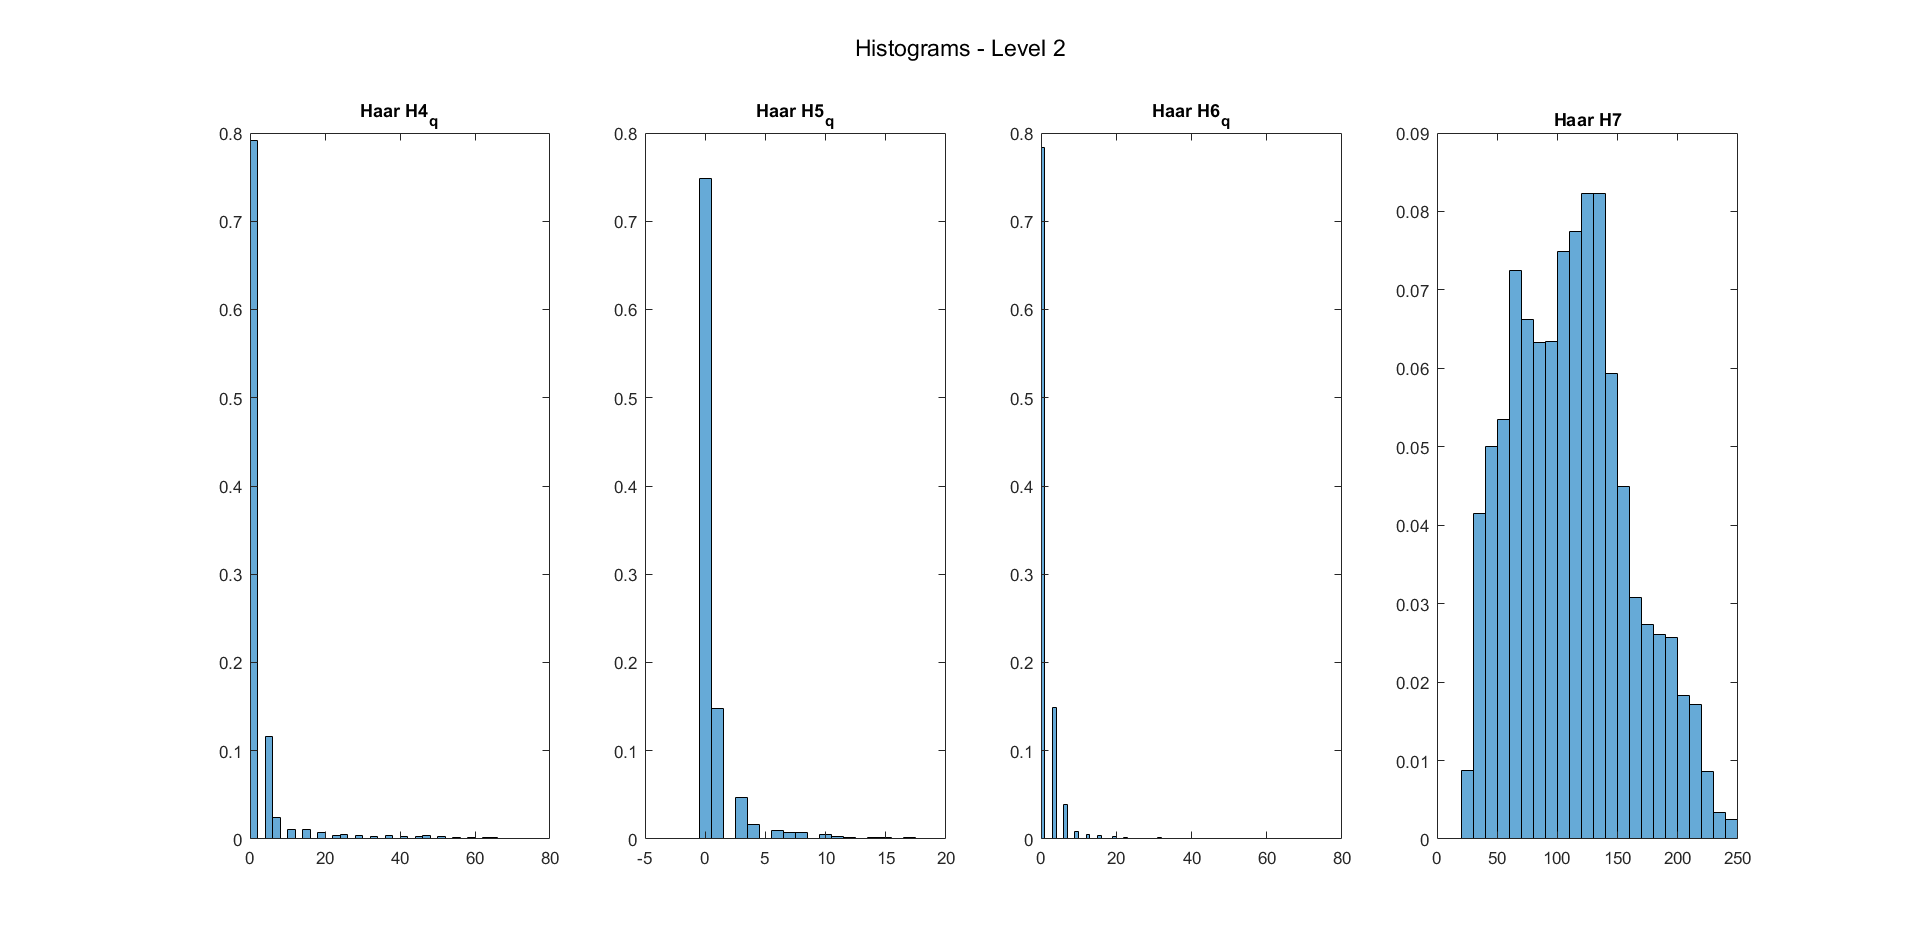
\includegraphics[height=5cm, width=\linewidth]{partC_lvl2_hists2.png}
		\end{subfigure}
	\end{figure}

	\noindent
	Αφού υπολογίστηκε η εντροπία κάθε κβαντισμένου subband, αθροίστηκαν ολες αυτές οι εντροπίες, για να προκύψει η συνολική της εικόνας μετά την εφαρμογή του μετασχηματισμού Haar και τη κβάντιση. Η συνολική τιμή της εντροπίας που προέκυψε για R=3 και R=5 είναι 4.5103 bits/pixel. Στη συνέχεια, μετά την ανακατασκευή, υπολογίστηκε η τιμή του peak SNR να είναι -11.785 ενώ το SNR είναι 30.0013 dB.\\
	
	\noindent
	Οι τελικές εικόνες που προκύπτουν μετά την ανακατασκευή είναι η εξής
	\begin{figure}[h!]
		\centering
		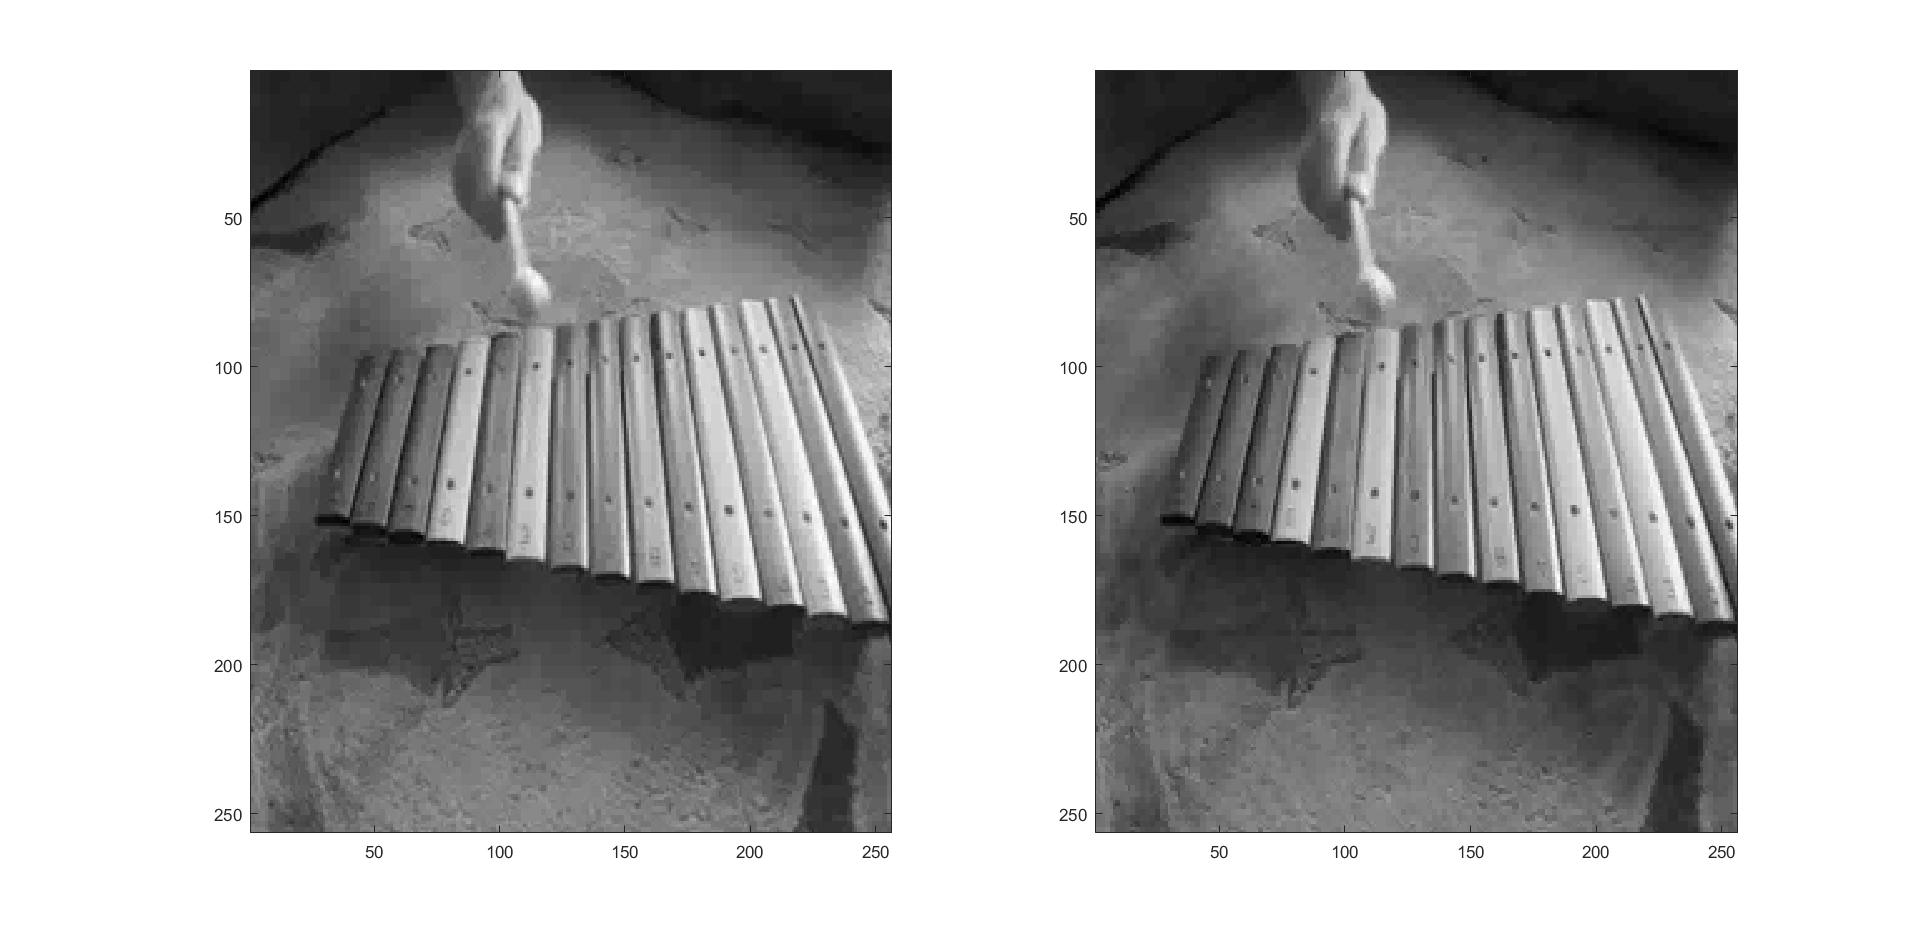
\includegraphics[height=5cm, width=\linewidth]{partC_R4_reconstructed.png}
		\caption{R=4 for both lvls of Haar (left) - R=3 for lvl 1 and R=5 for lvl 2 of Haar (right) }
	\end{figure}

	\noindent
	Συγκρίνοντας τις δύο περιπτώσεις βλέπουμε ότι έχουμε μεγαλύτερο ποσοστό συμπίεσης στην περίπτωση που χρησιμοποιούμε R=4 και στα 2 επίπεδα του μετασχηματισμού Haar. Αυτό επαληθεύεται και από την εντροπία όπου στην πρώτη περίπτωση είναι 3.9434 bits/pixel, ενώ στη δεύτερη περίπτωση αυξάνεται και είναι 4.5103 bits/pixel. Αυτή η αύξηση της εντροπίας είναι λογική, καθώς στην πρώτη περίπτωση για R=4 και στα δύο επίπεδα χρησιμοποιούμε συνολικά $2 \cdot 2^4 = 32$ επίπεδα κβάντισης, ενώ στη δεύτερη περίπτωση χρησιμοποιούμε  $2^3 + 2^5 = 8 + 32 = 40$ επίπεδα κβάντισης. Τέλος, όσον αφορά τα Peak SNR βλέπουμε ότι στη δεύτερη περίπτωση το peak SNR, καθώς και το πραγματικό SNR έχουν μειωθεί σε σχέση με την πρώτη περίπτωση που χρησιμοποιούμε το ίδιο R και στα δύο επίπεδα του μετασχηματισμού Haar.
\end{document}
